\documentclass[12pt]{article}

\usepackage{amsmath,amssymb,amsthm}
\usepackage{graphicx}
\usepackage{hyperref}
\usepackage{float}
\usepackage[most]{tcolorbox}
\usepackage{booktabs}
\usepackage{tabularx}
\usepackage{caption}
\usepackage{placeins}
\usepackage[margin=1in]{geometry}

\renewcommand{\topfraction}{0.9}
\renewcommand{\bottomfraction}{0.8}
\renewcommand{\textfraction}{0.05}
\renewcommand{\floatpagefraction}{0.75}
\setcounter{topnumber}{3}
\setcounter{bottomnumber}{2}
\setcounter{totalnumber}{5}

% Supplementary numbering
\renewcommand{\thesection}{S\arabic{section}}
\renewcommand{\thesubsection}{S\arabic{section}.\arabic{subsection}}
\renewcommand{\thesubsubsection}{S\arabic{section}.\arabic{subsection}.\arabic{subsubsection}}
\renewcommand{\thetable}{S\arabic{table}}
\renewcommand{\thefigure}{S\arabic{figure}}
\renewcommand{\theequation}{S\arabic{equation}}

\title{Repository notes for\\
\emph{Chromatically Constrained Tensor Graphs: Concurrency and Connectome Topology}}
\author{Vahid R. Ramezani \and Benjamin Englard}
\date{}

\begin{document}
\sloppy
\maketitle

\noindent
These notes contain the detailed construction procedures,
parameter accounting, null-model definitions, extended graph audits, and
computational-model specifications underlying the main article. The main text
now emphasizes two comparatively simple constructions: the local
prune--repair construction and the $8{,}000$-node seed-encoded construction.
These notes give reproducibility details for those models and
retains the earlier, more elaborate $16{,}807$-node fixed-partition relocation
pipeline as an optional refinement for the case in which fiber-bundle
multiplicity is itself treated as an explicit target. The organization
separates reproducibility-oriented methods from extended results that are
summarized more compactly in the main text.

\section{Supplementary Methods}
\label{supp:methods}

\subsection{Local construction and quotienting}

In this section we show that a simple two-part algorithm with a small number
of parameters can produce a graph that matches numerous properties of the
connectome reported across the literature.

The main article next introduces a second, simpler construction in which a
four-block mesoscale template is encoded directly in a $20$-vertex seed and
propagated by tensor growth. We give its exact reproducibility details below.
A later supplementary subsection then retains the older, more elaborate
fixed-partition relocation pipeline. That pipeline is no longer the principal
second construction; it is included because it demonstrates how the
fiber-bundle distribution can be matched when that statistic is targeted
explicitly.

A small tripartite seed is expanded repeatedly by tensor product.  After
each expansion, the graph is pruned, locally repaired, and closed by
chromatically legal triangle additions.  Finally, the resulting parent graph
is coarsened to a \(1{,}015\)-node quotient.

\begin{tcolorbox}[
breakable, colback=white, colframe=black, boxrule=0.5pt, arc=0pt,
left=6pt, right=6pt, top=6pt, bottom=6pt,
title={Algorithm 1A: Parent construction by local repair}
]
\small

\textbf{Input.}
A tripartite seed graph \(S=(V_S,E_S)\) with proper 3-coloring
\(c_S:V_S\to\{0,1,2\}\); tensor depth \(K\); minimum degree \(d_{\min}\);
pruning fraction \(p\); triangle-addition fraction \(a\); and a fixed random
seed for randomized tie-breaking.

\medskip
\textbf{Definitions.}
At scale \(k\), let \(n_k=|V(G_k)|\) and define the geometric-mean edge budget
\[
b_k
=
\operatorname{round}\!\left(
n_k\sqrt{\frac{n_k-1}{2}}
\right).
\]
A legal edge is an edge \(\{x,y\}\) satisfying \(c(x)\ne c(y)\).  Only legal
edges are added; deletions are unrestricted.  The triangle support of an
edge \(\{u,v\}\) is \(|N(u)\cap N(v)|\).

\medskip
\textbf{Initialize.}
\(G_0=S\), \(c=c_S\).

\medskip
For \(k=0,1,\ldots,K-1\), perform the following steps.

\begin{enumerate}

\item \textbf{Tensor expansion.}
Set \(\widetilde G_{k+1}=G_k\otimes S\).  The vertices of
\(\widetilde G_{k+1}\) are pairs \((u,a)\), where \(u\in V(G_k)\) and
\(a\in V_S\).  An edge joins \((u,a)\) and \((v,b)\) exactly when
\(\{u,v\}\in E(G_k)\) and \(\{a,b\}\in E_S\).  Project the coloring
according to \(c((u,a))=c(u)\).  Thus every tensor edge remains cross-color,
and the proper 3-coloring is preserved.  Because $G_k$ and $S$ are connected
and non-bipartite, $\widetilde G_{k+1}$ is also connected and non-bipartite;
record one odd cycle $C_{k+1}$ before pruning as an invariant witness.

\item \textbf{Community-aware pruning.}
Score every edge of \(\widetilde G_{k+1}\) by its triangle support.  Retain
the \(\operatorname{round}(p\,b_{k+1})\) highest-support edges and delete the
remaining edges.

\item \textbf{Local chromatic repair.}
For each vertex whose degree is below \(d_{\min}\), add legal cross-color
edges through the vertex's two-hop neighborhood whenever possible,
preferentially selecting edges that close local triangles.  If the local
candidate pool is exhausted, use any available legal endpoint.  If the graph
is disconnected, add legal bridging edges until connectivity is restored.

\item \textbf{Chromatic triangle closure.}
For every open wedge \(u-v-w\), admit the closing edge \(\{u,w\}\) as a
candidate only when \(c(u)\ne c(w)\).  Rank the candidate closures by
common-neighbor support and add them until the total edge count reaches
\(\operatorname{round}(a\,b_{k+1})\).

\item \textbf{Invariant safeguard.}
Verify connectivity and non-bipartiteness of the edited graph.  If it is
disconnected, add legal cross-color bridging edges until connectivity is
restored.  If it is bipartite, restore any tensor edges of the recorded odd
cycle \(C_{k+1}\) that were deleted during this stage until the whole cycle is
present again.  These restored tensor edges are cross-color under the
projected coloring.  The invariant safeguard takes precedence over the
nominal edge-count target.

\end{enumerate}

Set \(G_{k+1}\) equal to the resulting graph.  After \(K\) tensor steps,
\(G_K\) is the parent graph.

\medskip
\textbf{Output.}
The locally repaired parent graph \(G_K\), together with its proper
3-coloring \(c\).

\end{tcolorbox}

\begin{tcolorbox}[
breakable, colback=white, colframe=black, boxrule=0.5pt, arc=0pt,
left=6pt, right=6pt, top=6pt, bottom=6pt,
title={Algorithm 1B: Coarsening to the quotient}
]
\small

\textbf{Input.}
The parent graph \(G_K\) produced by Algorithm~1A; Louvain resolution
\(\gamma\); target quotient size \(N\); and a fixed random seed.

\medskip
\textbf{Definitions.}
For two communities \(A\) and \(B\), let \(w(A,B)\) denote the number of
edges of \(G_K\) with one endpoint in \(A\) and the other in \(B\).  Define
their intercommunity edge density by
\(\rho(A,B) = w(A,B)/(|A|\,|B|)\).

\medskip
\begin{enumerate}

\item \textbf{High-resolution partition.}
Run Louvain community detection on \(G_K\) at resolution \(\gamma\), chosen
so that the number of detected communities exceeds the target \(N\).

\item \textbf{Density-based merging.}
While the number of communities is greater than \(N\), choose a smallest
community \(A\).  Among the communities adjacent to \(A\), select a
community \(B\) maximizing \(\rho(A,B)\), and merge \(A\) into \(B\).
Continue until exactly \(N\) supernodes remain.

\item \textbf{Quotient construction.}
Construct the quotient graph \(H_{\rm LR}\) with one vertex for each
surviving supernode.  Two distinct supernodes are adjacent in
\(H_{\rm LR}\) if and only if at least one edge of \(G_K\) has endpoints in
the two corresponding communities.

\end{enumerate}

\medskip
\textbf{Output.}
The local quotient \(H_{\rm LR}\).

\end{tcolorbox}

For the concrete run reported here, the seed has \(|V_S|=7\) vertices and
\(|E_S|=9\) edges.  We use tensor depth \(K=4\), minimum degree
\(d_{\min}=3\), pruning fraction \(p=0.10\), triangle-addition fraction
\(a=0.18\), Louvain resolution \(\gamma=40\), target quotient size
\(N=1{,}015\), and random seed \(42\).  With these values, the local
construction produces a quotient \(H_{\rm LR}\) with
\[
n=1{,}015,\qquad |E|=67{,}094,\qquad \rho=0.1304,\qquad Q=0.524.
\]

This is the whole local construction.  It has no empirical adjacency matrix,
no anatomical coordinates, no tractography weights, no fitted edge
probabilities, no later fixed-partition inverse-relocation stage.  It is a local
growth-and-repair mechanism followed by quotienting.  Only node count, edge
count, modularity, and low-degree nodes were used as targets.


\paragraph{Edge-budget normalization.}
The local construction was initially parameterized from the side of graph
complexity.  For a graph on \(n\) vertices, the sparsest connected graph has
\(O(n)\) edges, while the complete graph has \(n(n-1)/2\) edges.  Many graph
complexity measures are small near both extremes: trees and paths are too
regular, while complete graphs are also highly regular.  The natural
intermediate scale is therefore the geometric mean between the sparse
connected scale and the complete-graph scale,
\[
E_{\rm gm}
=
n\sqrt{\frac{n-1}{2}},
\]
up to the immaterial distinction between using \(n\) and \(n-1\) for the
sparse connected reference.  This is the edge scale associated with maximal
graph complexity in several graph-complexity measures
\cite{KimWilhelm2008ComplexGraph}.

In the local construction we did not use the full complexity scale.  We used
a fraction of it, \(E_{\rm LR}=\alpha E_{\rm gm}\) with \(\alpha=0.18\).  At
the final parent size \(n=16{,}807\), this gives \(E_{\rm LR}=277{,}319\).
Thus the local graph lies well below the maximal-complexity scale.  This was
empirically necessary: pushing the budget closer to \(E_{\rm gm}\) produced
graphs that were too dense, too modular, and lost the low-degree periphery
seen in the Budapest graph.

The global construction uses the same sparse regime but expresses it from
the opposite direction.  Instead of taking a fraction down from the
maximal-complexity scale, it starts from the connectivity scale, of order
\(n\log n\), and works upward by a controlled multiple.  At \(n=16{,}807\),
the local budget \(277{,}319\) is already only \(1.18\,n\log_2 n\), or about
\(3.39\) times the classical connectivity threshold \(n\ln n/2\).





\subsection{Eight-thousand-node seed-encoded construction}
\label{supp:eightk-methods}

The second main construction is generated by a standalone procedure that does
not read an empirical adjacency matrix or any other graph file. It begins from
a hand-specified seed with $20$ vertices and $31$ edges. Each seed vertex has
an independent color label and block label. The color classes have sizes
$6/6/8$; the blocks $A,B,C,D$ have sizes $6/6/4/4$. Blocks $A,C$ form one
larger group and $B,D$ the other. Every seed edge is cross-color. The edge
inventory is $26$ within-block edges, four same-group cross-block edges, and
one edge between the two larger groups.

Growth uses tensor product with in-loop triangle closure:
\[
G_1=S+A_0,
\qquad
G_2=(G_1\otimes S)+A_1,
\qquad
G_3=(G_2\otimes S)+A_2,
\]
where $A_0$, $A_1$, $A_2$ are the legal closures made at the seed stage
and at scales two and three.
The final parent therefore has $20^3=8{,}000$ vertices. Closure is applied with
quotas
\[
\alpha=(3,4,30)
\]
and degree-weighting exponent
\[
\beta=1.5.
\]
For one candidate closure, a center vertex $v$ is sampled with probability
proportional to $\deg(v)^\beta$ and two neighbors $u,w$ are selected. The edge
$\{u,w\}$ is added if and only if
\[
c(u)\neq c(w),
\qquad
b(u)=b(w),
\qquad
\{u,w\}\notin E.
\]
No edge is removed at any stage. Selection inside the legal candidate pool is
unranked. This is deliberate: ranking all closures by common-neighbor support
was tested and concentrated additions too strongly in the densest local
neighborhoods, reducing blind block recovery.

The finished parent contains
\[
n=8{,}000,
\qquad
m=477{,}584,
\]
with color classes $2{,}400/2{,}400/3{,}200$ and blocks
$2{,}400/2{,}400/1{,}600/1{,}600$. Since tensor edges inherit the seed's
cross-color legality and every closure is filtered explicitly, no chromatic
repair step is required. The graph has zero monochromatic edges and contains a
triangle, so $\chi=3$ exactly. Topology-only Louvain recovery of the finished
parent returns the four blocks with $\mathrm{NMI}=\mathrm{ARI}=1.000$.

Coarsening is performed independently within each block.   Louvain is run at
   high resolution; the adjacent pair of communities with the largest
   intercommunity density is then repeatedly merged until the target counts
\[
307/306/201/201
\]
are reached. These four target counts are the only numerical quantities taken
from the Budapest reference in this construction. Supernodes are joined in
the quotient whenever at least one parent edge crosses between them; no
quotient thinning follows. The strict quotient therefore contains
\[
n=1{,}015,
\qquad
m=64{,}760.
\]

The simple construction deliberately leaves one important mismatch. If
$W_{AB}$ denotes the number of fine edges underlying quotient relation
$A$--$B$, then the mean bundle multiplicity is $6.885$ rather than Budapest's
$2.033$, and the Gini coefficient is $0.661$ rather than $0.305$. A sweep over
the final closure quota shows that thinning the parent cannot remove this tail
without simultaneously damaging block recovery. This is the motivation for
the optional complex refinement below.

\subsection{Optional complex fiber-bundle refinement: integrated parent, fixed causal partition, and inverse relocation}
\label{supp:global-methods}
\emph{Exploratory; not part of the main article's reported results.}

This section gives the implementation-level construction used for the
integrated parent and the final inverse quotient.  The crucial distinction
from the earlier forward-only description is that the reported inverse run
does \emph{not} optimize a new coarse map.  The original integrated
causal-dependency graph is clustered once, reduced to exactly \(1{,}015\)
supernodes, and that assignment is then held fixed while fine causal edges are
reorganized beneath it.

A key tool used throughout the construction is Louvain community detection,
a modularity-optimization heuristic for partitioning a graph into communities
\cite{Blondel2008}.  Here it is used algorithmically.  Because it is applied
directly to the fine causal-dependency graph, the resulting supernodes are
mesoscale populations derived from the organization of that causal substrate;
no anatomical identity is assigned to them.

\paragraph{Seed graph.}
The integrated construction begins from the same fixed tripartite seed graph
used in the local construction,
\[
S=(V_S,E_S),\qquad |V_S|=7,\qquad |E_S|=9,
\]
with colors
\[
(0,0,1,1,2,2,2)
\]
and seed edges
\[
(0,2),(0,5),(1,3),(1,4),(1,6),(2,5),(2,6),(3,4),(3,6).
\]
Every seed edge joins vertices of different colors.

\paragraph{Stage A: chromatic tensor-product expansion and pruning.}
Four tensor-product expansion steps are applied after the initial seed, giving
\[
n=7^{4+1}=16{,}807
\]
vertices.  A product vertex \((u,a)\) inherits the color of its parent
coordinate,
\[
c_k(u,a)=c_{k-1}(u),
\]
so every tensor edge remains cross-color.  Pruning is performed after each
expansion.  At current size \(n\), the reported edge budget is
\[
B(n)=\operatorname{round}\!\big(n\log_2(n)m_{\rm mult}\big),
\qquad m_{\rm mult}=1.0.
\]
A Louvain partition is computed with seed \(42\) and resolution \(1.0\).
Each edge receives score
\[
s_A(u,v)=T(u,v)+10^{-7}(\deg u+\deg v),
\qquad
T(u,v)=|\Gamma(u)\cap\Gamma(v)|,
\]
and the budget is split between inter-community and intra-community edges
with inter-community fraction \(\eta=0.35\).  Highest-scoring edges are
retained within each pool.  Minimum-degree repair then inserts chromatically
legal edges until every vertex has degree at least three, and disconnected
components, if any, are reconnected by legal cross-color edges.

After the four expansion steps and repairs, an additional
\[
1.2n=20{,}168
\]
chromatically legal triangle-closing edges are added.  The resulting graph has
\(16{,}807\) vertices and \(273{,}695\) edges.

\paragraph{Stage B: multiscale-local cross-community bridges.}
The box-covering step is used as a multiscale locality filter, inspired by
network box-covering methods \cite{Song2005,Song2007memb}.  For
\[
l_B\in\{3,4,5,6,7\},
\]
randomized greedy coverings are constructed using
\(\operatorname{dist}(c,x)<l_B\).  Multiple vertex orderings are tried and
the covering with the fewest boxes is retained.  If \(b_{l_B}(u)\) is the
box label of vertex \(u\), define
\[
\kappa(u)=\big(b_3(u),b_4(u),b_5(u),b_6(u),b_7(u)\big).
\]
A candidate bridge \((u,v)\) is allowed only when
\[
\kappa(u)=\kappa(v),\qquad
\operatorname{comm}(u)\neq\operatorname{comm}(v),\qquad
c(u)\neq c(v),\qquad
(u,v)\notin E.
\]
Valid candidates are shuffled with seed \(42\), and up to
\(84{,}000\approx5n\) are inserted.  The reported run reaches
\(357{,}695\) edges at this stage.

\paragraph{Stage C: multiscale-targeted sparsification.}
The bridge-enriched graph is sparsified while monitoring a descriptive
box-covering slope.  The internal stopping target is
\[
d_B\leq3.8.
\]
For this stage the membership rule is \(\operatorname{dist}(c,x)\leq l_B\)
and the tested scales are
\[
l_B\in\{2,3,4,5,6,8,10,12\},
\]
restricted to scales no larger than the measured diameter.  Edges are ranked
for removal by
\[
s_C(u,v)=100T(u,v)+\frac{1}{\deg(u)+\deg(v)+1}.
\]
Graph bridges are protected at the start of each sparsification round, and a
removal is skipped if it would reduce either endpoint below degree two.  Up
to \(20{,}000\) removals are attempted per round, with edge-count floor
\(m_{\min}=100{,}000\).  The resulting original integrated parent has
\[
n=16{,}807,\qquad m=337{,}983,
\]
and remains properly three-colored.

\paragraph{Stage D: fixed community-derived causal partition.}
Louvain community detection is applied directly to the original integrated
parent at resolution
\[
\gamma_{\rm init}=20.0
\]
with seed \(42\), initially producing approximately \(1{,}054\) communities.
These are reduced to exactly
\[
N=1{,}015
\]
by deterministic density-based merging.  At each step, a smallest community
\(C_i\) is merged into the adjacent community \(C_j\) maximizing
\[
\frac{\operatorname{edges}(C_i,C_j)}{|C_i|\,|C_j|}.
\]
If \(C_i\) has no external neighbor, it is merged into the smallest other
community.  Let
\[
\pi:V_{\rm parent}\to\{1,\ldots,1015\}
\]
denote the resulting assignment, and define the member set of supernode \(a\)
by
\[
V_a=\{u:\pi(u)=a\}.
\]
This map is fixed throughout all reported inverse stages.  Every fine vertex
therefore remains in the same causally derived supernode while the fine edge
set changes.

For any fine graph under this fixed map, define the complete cross-supernode
bundle
\[
E_{ab}=\{\{u,v\}\in E:\{\pi(u),\pi(v)\}=\{a,b\}\},\qquad a\neq b,
\]
with multiplicity \(W_{ab}=|E_{ab}|\).  The reported quotient is always
reconstructed by complete counting of these sets.

\paragraph{Forward strict-coarsening obstruction.}
Strict collapse of the unchanged integrated parent under this map yields
\(143{,}679\) cross-supernode relations, with modularity \(Q=0.124\),
clustering \(C=0.373\), and characteristic path length \(1.725\).  A sweep of
\(25\) additional strict coarsenings, all forced to \(1{,}015\) groups,
includes Leiden RB and CPM, balanced METIS, Louvain--METIS hybrids, nested
maps, box-covering maps, and a random balanced control.  The best modularity
observed is \(0.288\), still below Budapest's \(0.5574\).  The fixed-parent
forward problem therefore does not reach the target mesoscale regime.

\paragraph{Mesoscale target-support scaffold.}
The first inverse stage uses a stored target support set \(\mathcal S\) built
from the weighted witness graph of the original integrated parent.  This is a
construction scaffold, not a valid strict quotient of the unchanged parent.
Unweighted Louvain at resolution \(0.95\) gives four large blocks of sizes
\[
389,\quad265,\quad239,\quad122.
\]
All witness relations within each top-level block are retained.  Finer
within-block partitions are computed with
\[
\begin{array}{c|cc}
\text{block}&\gamma_{L1}&\gamma_{L2}\\
\hline
0&0.9&1.0\\
1&0.7&1.0\\
2&1.0&2.0\\
3&1.0&2.0
\end{array}
\]
and cross-top-block \(L1\)-group pairs are ranked by total witness weight.
The ten strongest cross-block patches are used, with individual relations
added in decreasing witness-weight order toward
\[
\left\lfloor\frac{139N}{2}\right\rfloor.
\]
The stored scaffold contains \(70{,}538\) relations.  It is used only as the
target support for the fine-edge redistribution below.

\paragraph{Stage E: bundle-weight redistribution.}
Starting from the original integrated parent, every current cross-supernode
pair absent from \(\mathcal S\) loses all of its fine support.  Let the pairs
in \(\mathcal S\) be sorted in ascending order of their original witness
multiplicity.  The implementation samples the same number of Budapest
\texttt{fiber\_count\_mean} values without replacement using seed \(42\),
sorts the sampled values, and assigns them rank-for-rank.  The integer target
multiplicity is
\[
t_p=\max\{1,\operatorname{round}(b_p)\}.
\]
For an overweight pair, supporting fine edges are scored by common-neighbor
support and the lowest-support edges are removed first.  For an underweight
pair \((a,b)\), absent cross-color edges with \(u\in V_a\) and \(v\in V_b\)
are ranked by common-neighbor support and the highest-scoring candidates are
added until the target multiplicity is reached.

Fine vertices below degree three are repaired first through legal two-hop
candidates ranked by common-neighbor support and then, if needed, by seeded
random legal non-neighbors.  Connectivity is restored by legal cross-color
edges if required.  Any remaining parent-edge deficit is then restored
inside supernodes, processing the largest supernodes first and preferring
absent cross-color pairs with high common-neighbor support.  The complete
strict quotient recomputed from this parent has \(71{,}696\) relations and
already passes the nine-criterion quotient audit.

\paragraph{Stage F: mesoscale support refinement.}
The complete strict quotient of the bundle-redistributed parent is partitioned
by unweighted Louvain at resolution \(0.95\).  Within the four largest blocks,
additional unweighted partitions use resolutions \(0.9,0.7,1.0,1.0\).
Existing relations lying in the same top-level block but different finer
groups are ordered by ascending bundle multiplicity, and the first
\(6{,}500\) are selected.  Removing a selected coarse relation means removing
\emph{all} fine parent edges supporting it.

Replacement candidates are quotient nonrelations whose endpoints lie in the
same finer group.  They are ranked by coarse common-neighbor count and the top
\(6{,}500\) are selected.  For each selected pair \((a,b)\), the implementation
searches only the first \(30\) stored members of \(V_a\) and the first \(30\)
stored members of \(V_b\).  Among legal missing cross-color edges in this
\(30\times30\) set, the candidate maximizing parent common-neighbor support is
inserted when one exists.  The fine parent is authoritative: only relations
with explicit fine support survive into the final stage.

\paragraph{Stage G: final degree-profile adjustment.}
The final adjustment starts from the parent produced above and uses NumPy seed
\(11\).  The complete strict quotient is reconstructed under the same fixed
map.  The Budapest degree sequence is sorted, and generated supernodes are
sorted by their current degree; target degrees are then assigned rank-for-rank.
No anatomical node correspondence is implied.

Supernodes above target are processed from largest surplus to smallest.
Incident quotient relations are considered in ascending bundle multiplicity,
and a relation is removed only when its partner is also above target.  When a
relation is removed, all of its supporting fine edges are deleted.  These
removed fine edges define the budget available for new cross-supernode
support.

Supernodes below target are processed from largest deficit to smallest.  Each
search attempt samples \(60\) supernode indices with replacement.  The first
sampled partner that is distinct, not already adjacent in the quotient, and
also below target is selected.  Stored member lists are scanned in order for
chromatically legal missing fine edges; the implementation can insert up to
two fine edges supporting the new coarse relation.  Any remaining parent-size
deficit is restored inside supernodes.  Bundle-rank assignment is not rerun
at this stage; final bundle statistics are measured from the completed
parent.

Approximately \(2{,}146\) fine-edge changes occur in this final degree-profile
adjustment.  The completed relocation substrate has
\[
16{,}807\ \text{vertices},\qquad337{,}980\ \text{edges},
\]
and its single final strict quotient has
\[
1{,}015\ \text{vertices},\qquad71{,}098\ \text{edges}.
\]

\paragraph{Reported-run parameters.}
\begin{table}[H]
\centering
\small
\setlength{\tabcolsep}{4pt}
\begin{tabularx}{\textwidth}{p{0.34\textwidth}X}
\toprule
Parameter & Role \\
\midrule
\(K=4\) & Tensor-product expansion steps. \\
\(m_{\rm mult}=1.0\) & Multiplier in \(B(n)=n\log_2(n)m_{\rm mult}\). \\
\(\eta=0.35\) & Inter-community fraction of the pruning budget. \\
\(\gamma_{\rm prune}=1.0\) & Louvain resolution during tensor-step pruning. \\
\(d_{\min}^{\rm repair}=3\) & Fine-vertex degree floor after pruning and during bundle repair. \\
\(\alpha_{\triangle}=1.2\) & Post-expansion triangle-closing budget. \\
\(\mathcal L_{\rm bridge}=\{3,4,5,6,7\}\) & Box scales used for bridge candidates. \\
\(\alpha_{\rm bridge}=5\) & Maximum bridge budget in units of \(n\). \\
\(d_B^*=3.8\) & Descriptive box-covering target during sparsification. \\
\(\mathcal L_{\rm sparse}=\{2,3,4,5,6,8,10,12\}\) & Scales used during sparsification. \\
\(N=1{,}015\) & Number of fixed supernodes. \\
\(\gamma_{\rm init}=20.0\), seed \(42\) & Original-parent community partition. \\
\(\gamma_0=0.95\) & Coarsest hierarchy resolution. \\
10 & Number of strongest cross-block \(L1\)-pair patches retained in the target scaffold. \\
seed \(42\) & Bundle-value sampling and bundle-stage repairs. \\
without replacement & Sampling rule for Budapest bundle values. \\
400 & Largest-component vertices scanned during connectivity repair. \\
\(6{,}500\) & Relations selected in mesoscale support refinement. \\
30 & Stored members examined per supernode when realizing a refinement-stage relation. \\
seed \(11\) & Final degree-profile adjustment. \\
60 & Candidate partner supernodes sampled per deficit-search attempt. \\
\(\approx2{,}146\) & Fine-edge changes in the final degree-profile adjustment. \\
\bottomrule
\end{tabularx}
\caption{Parameters and deterministic search limits used in the reported integrated and inverse construction.}
\label{tab:reported-run-parameters}
\end{table}

The node count, coarse edge scale, degree distribution, and bundle-weight
distribution are explicit constraints on the inverse solution.  No individual
Budapest node, edge, or tract is fitted anatomically.

\subsection{Eight-thousand-node recurrent image-inpainting architecture}
\label{supp:eightk-inpainting}

The main article's current computational realization uses the $8{,}000$-node
parent rather than the complex relocation substrate. The task is
$256\times256$ CelebA-HQ image inpainting. A convolutional encoder takes RGB
plus a binary mask and produces six feature maps:
\[
64\times256\times256,
\quad
128\times128\times128,
\quad
256\times64\times64,
\]
\[
512\times32\times32,
\quad
512\times16\times16,
\quad
512\times8\times8.
\]
All six encoder levels are sent to the graph. A collector pools and projects
them to channel width $C=32$ and assigns exactly $2{,}400$ feature slots to
the first color class. On the $8{,}000$-node substrate the slot counts are
$512,128,32,1{,}024,480,224$ for encoder levels
$s_3,s_4,s_5,s_2,s_1,s_0$, respectively, summing exactly to $2{,}400$.

Every fine graph edge supplies a fixed sparse routing location whose scalar
weight is learned. Five sparse operators are used:
\[
1\to2,
\qquad
1\to3,
\qquad
2\to3,
\qquad
3\to2,
\qquad
3\to1.
\]
The two feedback masks are transposes of the corresponding forward masks but
carry independent trainable weights. The model executes five recurrent passes.
Population $a_2$ is computed from the old $a_1$ plus delayed $a_3\to a_2$
feedback; $a_1$ is then re-anchored to the encoder-derived base state plus
$a_3\to a_1$ feedback; $a_3$ is recomputed from the fresh $a_1$ and current
$a_2$. This produces a recurrent rather than feed-forward use of the three
color classes.

Same-phase coactivation is modeled separately by shared linear-attention
blocks operating within each non-empty (color, supernode) group. Attention
therefore mixes nodes inside a causal phase without introducing same-color
edges into the structural graph. The decoder readout uses all $3{,}200$ nodes
of the third color class. Learned projections over all third-class nodes
produce the two deepest decoder inputs ($8\times8$ and $16\times16$), while
four exact node blocks from the final recurrent pass produce the remaining
multiscale graph features. The graph replaces the ordinary U-Net bottleneck
and the two deepest skips; the three shallow convolutional skips remain and
are modulated by graph-derived features.

The graph-plus-attention model contains $74{,}911{,}834$ parameters on the
$8{,}000$-node substrate, compared with $87{,}103{,}619$ for the matched U-Net
baseline. The graph's five sparse operators account for $806{,}871$ trainable
parameters and the same-phase attention blocks for $12{,}864$.

The final comparison uses three independently trained seeds per model under
the same train/validation split, mask generator, optimizer, and checkpoint
rule; the evaluation protocol and results are reported in the main article.

\subsection{Auxiliary image-inpainting results on the 16,807-node relocation substrate}
\label{supp:inpainting-methods}
\emph{Exploratory; not part of the main article's reported results.}

This subsection is retained from the earlier complex-substrate experiment. It is useful as an auxiliary demonstration that the larger relocation graph can be trained end to end, but it is no longer the primary computational experiment in the main article. The primary architecture now uses the $8{,}000$-node substrate described immediately above.

\paragraph{Task and data.}
We evaluate the graph module in a \(256\times256\) CelebA-HQ image-inpainting
task. Each example contains an image \(x\), a binary mask \(m\), and the
masked observation
\[
x_{\rm obs}=m\odot x.
\]
The model receives the four-channel tensor \([x_{\rm obs},m]\) and predicts a
raw reconstruction \(\hat x\). The reported composite preserves the observed
pixels,
\[
\hat x_{\rm final}
=
m\odot x_{\rm obs}+(1-m)\odot\hat x.
\]

Training uses \(28{,}000\) images with \(2{,}000\) held out. The same
irregular-mask routine is used for training and evaluation, but with different
target-coverage distributions. During training, the target coverage is sampled
from
\[
U(0.09,0.49).
\]
Across \(30{,}000\) generated training masks, the achieved missing fractions
span approximately
\[
[0.0904,0.6040].
\]
The broader benchmark instead samples target coverage from
\[
U(0.02,0.70).
\]
Of the \(4{,}893\) benchmark masks entering the scored coverage buckets,
\(579\) (\(11.8\%\)) fall outside the achieved training range. All of these
lie below the training floor and within the \(0\)--\(20\%\) coverage band;
the \(20\)--\(40\%\) and \(40\)--\(60\%\) bands lie within the achieved
training range.

The benchmark-mask distribution is the primary reported evaluation because it
is the protocol used for comparison with the matched U-Net baseline.
Evaluation on the training-mask distribution is reported as a robustness
check. Aggregates from the two mask distributions are not interpreted as a
direct performance comparison because the distributions populate the six
coverage buckets differently.


\paragraph{Architecture and graph substrate.}
The recurrent model operates directly on the final substrate, obtained after
bundle-matching relocation, mesoscale support refinement, and degree matching:
\[
n=16{,}807,\qquad
m=337{,}980,\qquad
\chi=3,
\]
with fixed color-class sizes
\[
n_1=4{,}802,\qquad
n_2=4{,}802,\qquad
n_3=7{,}203.
\]
The fixed \(1{,}015\)-supernode assignment is retained as the mesoscale
grouping used by the optional supernode-attention modules. There is no
separate reconstruction of a fine graph from the quotient before training.

The graph model replaces the ordinary deepest encoder--decoder pathway with a
collector, sparse recurrent graph, and multiscale graph-to-decoder readout.
The encoder produces feature maps
\[
s_0,s_1,s_2,s_3,s_4,s_5
\]
at spatial resolutions
\[
256,\ 128,\ 64,\ 32,\ 16,\ 8
\]
with channel dimensions
\[
64,\ 128,\ 256,\ 512,\ 512,\ 512,
\]
respectively. The graph-state width is \(C=32\).

The sparse forward operators are
\[
1\to2,\qquad
1\to3,\qquad
2\to3,
\]
with recurrent feedback
\[
3\to2,\qquad
3\to1.
\]
Sparse operators mix across graph nodes but not across feature channels. For
an allowed directed sparse operator,
\[
Y_{b,u,c}
=
b_u+
\sum_{v:\,v\to u\ {\rm allowed}}
\theta_{uv}X_{b,v,c},
\]
where \(\theta_{uv}\) is the learned scalar associated with an allowed graph
connection and \(b_u\) is the learned node bias. Absent graph connections
carry no sparse edge parameter.


\paragraph{Collector.}
Each encoder level is projected to graph width by a \(1\times1\) convolution
and flattened into node features. The allocation over the \(4{,}802\) nodes
of the first color class is
\[
\begin{array}{llr}
s_3:&32\times32&1024\\
s_4:&16\times16&256\\
s_5:&8\times8&64\\
s_2:&64\times64\to32\times64&2048\\
s_1:&128\times128\to30\times32&960\\
s_0:&256\times256\to18\times25&450
\end{array}
\]
in the order
\[
[s_3,s_4,s_5,s_2,s_1,s_0],
\]
summing exactly to \(4{,}802\) graph nodes.


\paragraph{Recurrent graph update.}
Let \(a_1,a_2,a_3\) denote the states of the three color classes. The
collector initializes
\[
a_1^0
=
\operatorname{LN}_1
\!\left(
\operatorname{Collector}(s_0,\ldots,s_5)
\right),
\qquad
a_3\leftarrow0.
\]
Each of five recurrent passes then applies
\[
a_2
=
\operatorname{GELU}\!\left(
\operatorname{LN}_2\!\left(
W_{12}a_1+
\operatorname{LN}_{fb}(W_{32}a_3)
\right)
\right),
\]
\[
a_1
=
a_1^0+
\operatorname{LN}_{fb1}(W_{31}a_3),
\]
and
\[
a_3
=
\operatorname{LN}_3
\!\left(
W_{23}a_2+W_{13}a_1
\right).
\]
When enabled, supernode attention is applied immediately after the
corresponding population update.

Attention is defined only for non-empty same-color groups under the fixed
supernode assignment. The median non-empty group contains \(3\) vertices in
each of the first two populations and \(4\) in the third, with means of
\(4.9\), \(4.8\), and \(7.1\), respectively. Pooled over all \(3{,}001\)
non-empty color--supernode groups, \(84.3\%\) contain eight vertices or fewer.
The largest groups in the three populations contain \(94\), \(102\), and
\(137\) vertices. Forty-four of the \(3{,}045\) possible color--supernode
slots are empty and therefore carry no attention block.

The update order is recurrent rather than a static feed-forward ordering.
In particular, \(a_2\) is computed before the \(3\to1\) feedback updates
\(a_1\), so the effect of that feedback reaches \(a_2\) on the following
recurrent pass. The implementation therefore selects one concrete causal
schedule for the three chromatic phase classes. The coloring fixes the minimum
number of phase classes required by the structural dependency graph; it does
not specify a unique temporal ordering. Dependencies may continue across
recurrent passes, so chromatic causal depth does not bound total computational
depth.


\paragraph{Twin path and decoder coupling.}
The graph state is mapped back into decoder features at six scales. The two
deepest outputs are learned projections over all \(n_3=7{,}203\) nodes and
are read from intermediate recurrent passes:
\[
t_5:\ 8\times8=64
\quad\text{from pass 3},
\]
\[
t_4:\ 16\times16=256
\quad\text{from pass 4}.
\]
The remaining four outputs are taken from the final recurrent pass:
\[
\begin{array}{llr}
t_3:&\to32\times32&1024\\
t_2:&\to32\times64\to64\times64&2048\\
t_1:&\to32\times64\to128\times128&2048\\
t_0:&\to32\times64\to256\times256&2048.
\end{array}
\]
The graph readout supplies the deep semantic pathway. At shallower levels the
ordinary encoder skips are retained and modulated by the corresponding graph
outputs.


\paragraph{Variant without attention.}
A variant removes only the three supernode-attention modules; everything
else is unchanged. It was run once.


\paragraph{Parameter counts.}
\begin{table}[H]
\centering
\small
\setlength{\tabcolsep}{5pt}
\renewcommand{\arraystretch}{1.08}
\begin{tabular}{@{}lrr@{}}
\toprule
Component
& Graph+attention
& Graph without attention\\
\midrule
Encoder
& \(26{,}108{,}928\)
& \(26{,}108{,}928\)\\
Decoder
& \(46{,}829{,}699\)
& \(46{,}829{,}699\)\\
Twin path
& \(2{,}370{,}752\)
& \(2{,}370{,}752\)\\
Sparse graph
& \(579{,}248\)
& \(579{,}248\)\\
Collector
& \(63{,}680\)
& \(63{,}680\)\\
Supernode attention
& \(12{,}864\)
& \(0\)\\
\midrule
Total
& \(75{,}965{,}171\)
& \(75{,}952{,}307\)\\
\bottomrule
\end{tabular}
\caption{Parameter accounting for the two graph-model variants. The final
substrate fixes the sparse routing pattern; training learns the parameters
carried by the allowed sparse operators. The matched U-Net baseline contains
\(87{,}103{,}619\) parameters.}
\label{tab:inpainting-parameters}
\end{table}


\paragraph{Training and checkpoint selection.}
All graph runs are trained from scratch for a fixed \(50\) epochs with AdamW,
batch size \(2\), gradient clipping at norm \(1.0\), and a cosine
learning-rate schedule decaying to zero. There is no early stopping.

Parameters in the encoder, decoder, and twin path use the base learning rate
\(3\times10^{-4}\) with weight decay \(10^{-4}\). The sparse-graph-plus-
collector group uses a \(10\times\) learning-rate multiplier,
\[
3\times10^{-3},
\]
with weight decay \(10^{-5}\). The U-Net comparison should therefore be
interpreted as an architecture-level computational comparison rather than as a
topology-only ablation.

Checkpoint selection follows a rule fixed before the final runs. Validation
loss is rounded to four decimal places; after epoch \(40\), the first sequence
of three consecutive epochs with the same rounded value is identified, and
the earliest checkpoint in that sequence is reported. All runs nevertheless
continue through the full \(50\) epochs.

For the three graph-plus-attention runs, this rule selects
\[
\text{seed 0: epoch 45},\qquad
\text{seed 1: epoch 44},\qquad
\text{seed 2: epoch 45}.
\]
For the three matched U-Net runs, the same rule selects
\[
\text{seed 0: epoch 47},\qquad
\text{seed 1: epoch 46},\qquad
\text{seed 2: epoch 46}.
\]
The single no-attention mechanism-check run selects epoch \(47\).

The pixel loss is
\[
\mathcal L_{\rm pix}
=
5\,\|(1-m)\odot(\hat x-x)\|_1
+
\|m\odot(\hat x-x)\|_1,
\]
with the observed-region term applied to the raw network output. A VGG16
perceptual loss on the hidden region is added with weight \(0.1\).
\paragraph{Three-seed graph evaluation.}
The primary graph evaluation uses benchmark masks with target coverage sampled
from \(U(0.02,0.70)\). Each metric is computed within six coverage buckets and
the six bucket values are then averaged. Thus the reported value is a mean of
bucket-level metrics rather than a direct per-image aggregate.

\begin{table}[H]
\centering
\small
\setlength{\tabcolsep}{5pt}
\renewcommand{\arraystretch}{1.08}
\begin{tabular}{@{}lrrrr@{}}
\toprule
Run
& L1 (\%)\,$\downarrow$
& PSNR\,$\uparrow$
& SSIM\,$\uparrow$
& LPIPS\,$\downarrow$\\
\midrule
Seed 0 (ep45)
& 1.4506 & 29.826 & 0.90403 & 0.09329\\
Seed 1 (ep44)
& 1.4539 & 29.823 & 0.90388 & 0.09349\\
Seed 2 (ep45)
& 1.4554 & 29.810 & 0.90369 & 0.09391\\
\midrule
Mean
& 1.4533 & 29.820 & 0.90387 & 0.09356\\
SD
& 0.0024 & 0.008 & 0.00017 & 0.00032\\
\bottomrule
\end{tabular}
\caption{Seed-level performance of the graph-plus-attention model on the
benchmark mask distribution. Values are means over the six coverage buckets
on the held-out reporting split. FID is omitted because it has not been
recomputed for the new three-seed graph experiment.}
\label{tab:inpainting-graph-seeds}
\end{table}

The same three graph-plus-attention checkpoints were also evaluated on the
training-mask distribution. The corresponding results are
\[
\begin{array}{lrrrr}
\toprule
\text{Run}
& \text{L1 (\%)}
& \text{PSNR}
& \text{SSIM}
& \text{LPIPS}\\
\midrule
\text{Seed 0 (ep45)}
&1.4099&29.352&0.90553&0.09179\\
\text{Seed 1 (ep44)}
&1.4152&29.346&0.90540&0.09200\\
\text{Seed 2 (ep45)}
&1.4154&29.343&0.90524&0.09243\\
\midrule
\text{Mean}
&1.4135&29.347&0.90539&0.09207\\
\text{SD}
&0.0031&0.005&0.00015&0.00033\\
\bottomrule
\end{array}
\]
The training-band aggregate should not be interpreted as an improvement over
the benchmark aggregate, because the two mask distributions populate the
coverage buckets differently. In the four central coverage buckets that are
well populated under both distributions, L1 differs by less than \(0.01\)
percentage points and PSNR by less than \(0.03\) dB across the measured runs.
In this toy example, a single run with the attention blocks removed
performed about the same as the attention-equipped model.

The matched U-Net remains the principal architectural baseline and is evaluated
under the benchmark-mask protocol. No U-Net result on the training-mask
distribution is inferred here. The inpainting experiment therefore supports
the narrower conclusion that the final fine graph can be instantiated as a
sparse recurrent computational substrate and trained reproducibly end to end;
it does not isolate the contribution of graph topology alone.

\subsection{Network-topology audit definitions and null models}
\label{supp:topology-methods}


We evaluate the generated graphs using a topology audit designed to test
whether a graph reproduces the main graph-theoretic signatures commonly reported
for structural brain networks.  The audit consists of nine scored criteria,
together with  unscored descriptive measures: box-covering scaling. Unless
stated otherwise, each scored comparison is evaluated against
degree-preserving null graphs generated by degree-preserving edge randomization, so that the result is not merely a consequence of the degree sequence
\cite{MaslovSneppen2002,VasaMisic2022}.  Enrichment criteria (clustering, modularity, local efficiency, and the significance clauses of the rich-club test) require the empirical value to exceed the null ensemble at \(p<0.05\), i.e.\ above the 95th percentile of the null distribution.

The descriptive box-covering and broad-degree checks are reported to
characterize the graph family, but they are not counted among the nine scored
quotient-level criteria.  This is especially important at the dense
\(1{,}015\)-node quotient scale, where graph distances are too compressed for
box-covering fits to be interpreted in the same way as on the large sparse
parent graph.



\paragraph{1. Clustering enrichment.}
Brain networks are locally clustered: neighbors of a node tend to be
connected to one another more often than in a comparable random graph.
We therefore require clustering, or transitivity, to be significantly
larger than the degree-preserving null ensemble. This captures the
segregated local structure emphasized in small-world network theory
\cite{WattsStrogatz1998}.  Clustering enrichment is not by itself a small-world criterion. Rather,
it measures the local-segregation component that distinguishes
small-world networks from ordinary random graphs. A graph is small-world
only when this local clustering is combined with near-random path length. 

\paragraph{2. Path length near random.}
Small-world organization also requires short global paths. We compare
the average shortest-path length of the graph to that of matched random
graphs and require it to remain close to random. Operationally, the audit
uses a tolerance of approximately 25 percent above the random-graph path
length. This prevents graphs from passing merely because they are highly
clustered but globally lattice-like.  Shortest-path quantities were computed exactly on the largest connected
component using sparse all-pairs shortest paths.  We used SciPy's
\texttt{csgraph.shortest\_path} routine with Dijkstra mode on the
unweighted, undirected adjacency matrix.  Average path length was
computed as the mean of all finite nonzero shortest-path distances.
Global efficiency was computed from the same distance matrix by averaging
reciprocal distances, with unreachable pairs contributing zero.



\paragraph{3. Small-world index.}
The small-world index combines the preceding two effects: clustering
should be much larger than random, while path length should remain near
random. We use the Humphries--Gurney statistic
\[
\sigma =
\frac{T/T_{\mathrm{null}}}{L/L_{\mathrm{null}}},
\]
where $T$ is transitivity and $L$ is average path length. The graph is
small-world when $\sigma>1$ \cite{HumphriesGurney2008}. We compute the
statistic against two null conventions: Erd\H{o}s--R\'enyi $G(n,m)$
graphs ($\sigma_{\mathrm{ER}}$, the scored criterion) and
degree-preserving edge-swap graphs ($\sigma_{\mathrm{dp}}$). Both are
reported; every graph audited in the main article satisfies $\sigma>1$
under both.

\paragraph{4. Modularity enrichment.}
Modularity enrichment measures whether the graph separates into
communities more strongly than expected from its degree sequence alone.
After community detection, each node $i$ is assigned a community label
$c_i$. For an undirected unweighted graph with adjacency matrix $A$,
degrees $k_i$, and total edge count $m$, the modularity of a partition is
\[
Q =
\frac{1}{2m}
\sum_{i,j}
\left(
A_{ij} - \frac{k_i\,k_j}{2m}
\right)
\mathbf{1}\{c_i=c_j\}.
\]
Here $A_{ij}$ records whether nodes $i$ and $j$ are connected, while
$k_i k_j/(2m)$ is the expected adjacency contribution between the same
two nodes under a degree-preserving configuration-model null. The
indicator $\mathbf{1}\{c_i=c_j\}$ restricts the sum to node pairs assigned
to the same community. Thus $Q$ is large when communities contain more
internal connectivity than would be expected from node degrees alone
\cite{NewmanGirvan2004}. In our audit, modularity enrichment passes only
when the detected partition has nontrivial modularity, $Q>0.3$, and the
observed value is significant against degree-preserving null graphs.



The community labels \(c_i\) are obtained by first applying a community
detection algorithm to the graph.  In our audit, we use Louvain community
detection, a modularity-optimization heuristic in the same community-detection
tradition as earlier large-network methods
\cite{ClausetNewmanMoore2004,Blondel2008}.  Thus \(c_i\) denotes the
Louvain community assigned to node \(i\).



\paragraph{5. Global efficiency near random.}
Global efficiency measures how efficiently information can travel across
the whole graph. If $d_{ij}$ denotes the shortest-path distance between
nodes $i$ and $j$, then
\[
E_{\mathrm{glob}}
=
\frac{1}{n(n-1)}
\sum_{i\neq j}
\frac{1}{d_{ij}} .
\]
Thus short paths contribute strongly, long paths contribute weakly, and
disconnected pairs contribute zero. We compare global efficiency with
matched degree-preserving null graphs. The criterion is not that global
efficiency should be maximized, but that it should remain close to random:
brain-like networks combine efficient long-range communication with
non-random local and modular structure. In our audit, this criterion
passes when $E_{\mathrm{glob}}/E_{\mathrm{glob,null}}$ lies in the range $[0.8,1.0)$ (near but below one) \cite{LatoraMarchiori2001,IturriaMedina2008}.





\paragraph{6. Local efficiency enrichment.}
Local efficiency measures how efficiently the neighbors of a node can
communicate with one another after that node is removed. For each node
$i$, let $N(i)$ be its neighborhood and let $G_i$ be the subgraph induced
by $N(i)$. The local efficiency of the whole graph is
\[
E_{\mathrm{loc}}(G)
=
\frac{1}{n}
\sum_{i=1}^{n}
E_{\mathrm{glob}}(G_i),
\]
where
\[
E_{\mathrm{glob}}(G_i)
=
\frac{1}{k_i(k_i-1)}
\sum_{\substack{j,h \in N(i)\\ j\neq h}}
\frac{1}{d^{(i)}_{jh}} .
\]
Here $k_i$ is the degree of node $i$, and $d^{(i)}_{jh}$ is the
shortest-path distance between neighbors $j$ and $h$ inside the
neighbor-induced subgraph $G_i$. If $k_i<2$, the contribution of node
$i$ is taken to be zero. Thus local efficiency is high when the neighbors
of a node remain well connected even without that node. We require local
efficiency to be enriched relative to degree-preserving null networks,
indicating more local fault-tolerant neighborhood structure than expected
from the degree sequence alone \cite{LatoraMarchiori2001}.

\paragraph{7. Connector hubs.}
Connectomes contain hubs that link multiple communities. After community
detection, let $c_i$ be the community of node $i$, let $k_i$ be its total
degree, and let $k_{is}$ be the number of edges from node $i$ to
community $s$. The participation coefficient of node $i$ is
\[
P_i
=
1 -
\sum_s
\left(
\frac{k_{is}}{k_i}
\right)^2 .
\]
This quantity is small when most edges of node $i$ remain inside one
community, and large when its edges are distributed across several
communities. We also compute the within-module degree score
\[
z_i
=
\frac{k_i^{\mathrm{in}}-\mu_{c_i}}{\sigma_{c_i}},
\]
where $k_i^{\mathrm{in}}$ is the number of edges from node $i$ to nodes
inside its own community, and $\mu_{c_i}$ and $\sigma_{c_i}$ are the mean
and standard deviation of within-community degree among nodes in the same
community as $i$. Following the Guimera--Amaral cartographic
classification, we call node $i$ a connector hub when
\[
z_i \geq 2.5
\qquad\text{and}\qquad
0.30 < P_i \leq 0.75 .
\]
Thus connector hubs are nodes that are hub-like inside their own module
while also linking substantially to other modules. The presence of at
least one such connector hub is used as evidence of cross-module
integration \cite{Guimera2005}.

\paragraph{8. Rich-club organization.}
Rich-club organization tests whether high-degree nodes are more densely
interconnected with one another than expected under a null model. For a
degree threshold $k$, let $N_{>k}$ be the number of nodes with degree
greater than $k$, and let $E_{>k}$ be the number of edges among those
nodes. The rich-club coefficient is
\[
R(k)
=
\frac{2E_{>k}}{N_{>k}(N_{>k}-1)} .
\]





This is the edge density of the subgraph induced by nodes whose degree
exceeds $k$. To test whether this density is larger than expected from
the degree sequence alone, we normalize by a degree-preserving null
ensemble:
\[
\rho(k)=\frac{R(k)}
{\langle R_{\mathrm{null}}(k) \rangle}.
\]
A value $\rho(k)>1$ means that high-degree nodes are more
interconnected than in matched null graphs. In our audit, rich-club
organization passes when $R_{\mathrm{norm}}(k)>1$ with statistical significance over a run of at least three consecutive degree thresholds, indicating a supported high-degree backbone \cite{Colizza2006,vandenHeuvel2011}.

\paragraph{9. Multi-resolution VI stability.}

This criterion follows the multi-scale brain-network view that community
structure should be examined across topological scales rather than at a
single fixed resolution \cite{BetzelBassett2017}; variation of information
provides the partition-distance measure used to identify reproducible
scales \cite{Meila2007}.

Hierarchical modular organization is tested by applying Louvain community
detection at several resolution parameters $\gamma$. The resolution
parameter controls the scale of the detected communities: smaller values
favor larger communities, while larger values favor smaller communities.
At each fixed value of $\gamma$, we repeat Louvain several times with
different random seeds. These repeats test whether the community structure
at that particular resolution is reproducible.

We compare the repeated community partitions using variation of
information,

\[
\mathrm{VI}(\mathcal{P},\mathcal{Q})
=
H(\mathcal{P})
+
H(\mathcal{Q})
-
2I(\mathcal{P};\mathcal{Q}),
\]

where $\mathcal{P}$ and $\mathcal{Q}$ are two detected community
partitions, $H$ denotes partition entropy, and $I$ denotes mutual
information. Low VI means that repeated runs found similar community
assignments. We then look across the tested values of $\gamma$ for local
minima of the mean VI. A local minimum identifies a resolution at which
the community structure is especially reproducible. We count such a
scale only when the corresponding modularity is also nontrivial, with
$Q>0.3$ \cite{Meila2007,Betzel2017modular}. The criterion passes when at
least one VI-stable modular scale is present.



\paragraph{10. Box-covering scaling (descriptive).}
Box covering asks how many boxes of a given size are needed to cover a graph.
For a box size \(l_B\), let \(N_B(l_B)\) be the number of boxes in a covering;
where the count follows a power law over a range of sizes, the box-covering
dimension is the negative slope
\[
d_B
=
-\,\frac{d\log N_B(l_B)}{d\log l_B},
\]
fitted by least squares on \(\log N_B\) against \(\log l_B\)
\cite{Song2005,Song2007memb}.  Exact minimum box covering is NP-hard, so the
count is always obtained by an approximation.  This work uses two different
approximations in two different roles, and they are not interchangeable; both
are given below.

\emph{(a) In the audit, as a measurement.}  Box counts are obtained by the
maximum-excluded-mass burning (MEMB) algorithm of Song et al.\
\cite{Song2007memb}, run on the exact all-pairs shortest-path matrix \(d\) of
the largest connected component.  For a burning radius \(r_B\):

\begin{enumerate}
\item Initialise every vertex as uncovered and as a non-centre.  For each
vertex \(u\), set its excluded mass
\(\mathrm{mass}(u)=|\{v: d(u,v)\le r_B\}|\).
\item While some vertex is neither covered nor a centre:
  \begin{enumerate}
  \item Among all non-centre vertices --- including those already covered,
        following Song's step (ii) --- select the vertex \(c\) of maximum
        excluded mass.
  \item If that maximum is zero, give each remaining uncovered non-centre
        vertex its own box and stop.
  \item Mark \(c\) a centre.  Assign to its box every uncovered vertex \(v\)
        with \(d(c,v)\le r_B\), mark those vertices covered, and increment the
        box count.
  \item For every vertex \(u\), reduce \(\mathrm{mass}(u)\) by the number of
        newly covered vertices within \(r_B\) of \(u\); set the mass of every
        centre to zero.
  \end{enumerate}
\item Report \(N_B(l_B)\) as the resulting box count, with box size
\(l_B=2r_B\).
\end{enumerate}

The procedure is deterministic: no random choices enter it.  Burning within
radius \(r_B\) bounds pairwise distances inside a box by \(2r_B\), which is
why \(l_B\) is defined as \(2r_B\); Song's text writes \(l_B=2r_B+1\) under a
strict distance bound, and we take the offset that reproduces the published
benchmark values more closely.  Step 3 is repeated for
\(r_B=1,\dots,\lfloor \mathrm{diam}/2\rfloor\), so the audited scales are
even.  Scales at which the graph is covered by a single box are discarded,
the remaining points are fitted in log--log to give \(d_B\), and an
exponential \(N_B \propto e^{-\beta l_B}\) is fitted to the same points for
comparison.  This is the only place \(d_B\) is measured.  It is descriptive
and is not one of the nine scored criteria: it is reported to characterize the
graph rather than to assert fractality, and only where the graph affords
enough distance range for a fit.

\emph{(b) In the construction, as a mechanism.}  The fractal-targeted
sparsification stage covers the graph in boxes in order to impose a property
rather than to measure one: edges of low triangle support are removed until
the stage's own estimate of \(d_B\) falls to its threshold.  Its covering is a
randomized greedy approximation, not MEMB.  For a scale \(l_B\):

\begin{enumerate}
\item Repeat for \(30\) independent trials:
  \begin{enumerate}
  \item Draw a uniformly random permutation of the vertices; mark all
        vertices uncovered and set the box count to zero.
  \item Scan the permutation in order.  Skip a vertex if it is already
        covered.  Otherwise take it as a centre \(c\), mark covered every
        vertex \(v\) with \(d(c,v)\le l_B\), and increment the box count.
  \item Stop the scan once every vertex is covered.
  \end{enumerate}
\item Take \(N_B(l_B)\) to be the smallest box count over the \(30\) trials.
\end{enumerate}

This is repeated over the scales \(\{2,3,4,5,6,8,10,12\}\), restricted to
those not exceeding the graph diameter; single-box scales are discarded and
the remaining points fitted in log--log as above.  Two differences from (a)
are worth making explicit.  Centres are taken in random order rather than by
excluded mass, so the covering is a best-of-\(30\) heuristic rather than a
deterministic construction.  And the ball is taken at radius \(l_B\) itself,
not at \(l_B/2\): for the same numeric label, a box here has twice the radius
of a box in (a).  The bridge stage uses a covering of the same greedy kind
over the scales \(\{3,4,5,6,7\}\), differing in taking the strict ball
\(d(c,v)<l_B\) and in using \(50\) trials rather than \(30\); its box labels
are used solely as a multiscale locality filter on candidate edges --- no
dimension is fitted there.



Because the centre rule, the meaning of \(l_B\), and the scale set all differ,
the threshold at which sparsification halts and the dimension the audit
subsequently reports are not the same quantity, and the two should not be read
as a target and a miss.






\section{Supplementary Results}
\label{supp:results}

\subsection{Parent-graph audits}
\label{supp:parent-graphs}

The local construction, the original integrated parent, and the final
relocation substrate are distinct fine-scale graphs.  The inverse procedure
changes edge placement under the fixed \(1{,}015\)-supernode causal partition;
the final relocation substrate is the graph used directly by the recurrent
neural model.

\subsubsection{Local parent graph}
The local construction gives
\[
n=16{,}807,\qquad m=277{,}319.
\]
Against tripartite degree-preserving nulls it passes seven of the nine scored
criteria.  The two failures are the explicitly integrative criteria:
near-random path length and near-random global efficiency.  Clustering,
small-world sigma, modularity, local efficiency, connector hubs, rich-club
organization, and multi-resolution modular stability all pass.

\subsubsection{Original integrated parent graph}
\emph{Exploratory; not part of the main article's reported results.}
The original integrated parent has
\[
n=16{,}807,\qquad m=337{,}983,\qquad \rho=0.002393,
\]
with color-class sizes \(4{,}802/4{,}802/7{,}203\).  Against \(1{,}000\)
tripartite degree-preserving nulls it passes all nine scored criteria.  Its
principal values are
\[
C=0.0366,\quad T=0.0317,\quad Q=0.4605,\quad
E_{\rm loc}=0.1208,
\]
\[
L=3.7871,\quad E_{\rm glob}=0.2844,\quad
\sigma_{\rm dp}=1.68,\quad\sigma_{\rm ER}=10.24,
\]
with assortativity \(+0.2542\).  The longest significant rich-club run is
\(290\).  The descriptive box-covering fit is
\[
d_B=4.03,\qquad R^2=0.94,
\]
and is not part of the nine scored criteria.

\subsubsection{Final relocation substrate}
\emph{Exploratory; not part of the main article's reported results.}

The final relocation substrate has
\[
n=16{,}807,\qquad m=337{,}980.
\]
It shares \(50.3\%\) of its edges with the original integrated parent, for
edge-set Jaccard similarity \(0.336\).  Its local and mesoscale organization
is substantially stronger:
\[
C=0.2281,\quad T=0.3089,\quad E_{\rm loc}=0.3497,
\quad Q=0.8104,
\]
with assortativity \(+0.5802\),
\[
\sigma_{\rm dp}=15.37,\qquad \sigma_{\rm ER}=83.80.
\]
Its average path length is \(4.5114\) and global efficiency is \(0.2439\).
Against \(1000\) tripartite degree-preserving nulls it passes seven of the nine
criteria, failing only the tests requiring path length and global efficiency
to remain near their randomized counterparts.  This is a near-randomness
failure rather than an absolute long-path regime: approximately \(93\%\) of
pairs are within six hops, the maximum observed hop distance is \(17\), and a
same-size ring lattice has average path length about \(210.6\).  The
descriptive box-covering fit is
\[
d_B=3.625,\qquad R^2=0.952.
\]
The recurrent neural model uses this final relocation substrate directly.



\subsection{Extended local-quotient analyses}
\label{supp:local-quotient}

\subsubsection{Local quotient topology audit}

After coarsening, the local quotient passes the same nine scored topology
criteria used below for the final quotient: clustering enrichment,
near-random path length, degree-preserving small-worldness, modularity
enrichment, near-random global efficiency, local efficiency enrichment,
connector hubs, rich-club organization, and multi-resolution VI-stable
modularity.

\begin{table}[htbp]
\centering
\small
\setlength{\tabcolsep}{4pt}
\renewcommand{\arraystretch}{1.05}
\caption{Nine-criterion topology audit for the local quotient
(\(n=1{,}015\), \(|E|=67{,}094\)) against the Budapest Reference Connectome.
Parenthetical values are ratios to degree-preserving null means.  Both
graphs pass all nine scored criteria.}
\label{tab:local-repair-nine-criteria}
\begin{tabularx}{\textwidth}{p{0.26\textwidth} X X c}
\toprule
Criterion & Local quotient & Budapest & Verdict \\
\midrule
Clustering enriched & \(C=0.515\)\,(\(2.46\times\)) & \(3.04\times\) & PASS \\
Path length near random & \(\mathrm{APL}=1.97\)\,(\(1.05\times\)) & \(1.19\times\) & PASS \\
Small-worldness (degree-pres.) & \(\sigma_{\mathrm{dp}}=2.30\) & \(\sigma_{\mathrm{dp}}=2.22\) & PASS \\
Modularity enriched & \(Q=0.524\)\,(\(8.24\times\)) & \(9.1\times\) & PASS \\
Global efficiency near random & \(E_{\mathrm{glob}}=0.548\)\,(\(0.97\times\)) & \(0.90\times\) & PASS \\
Local efficiency enriched & \(E_{\mathrm{loc}}=0.737\)\,(\(1.24\times\)) & \(1.38\times\) & PASS \\
Connector hubs & \(4\) hubs & \(4\) hubs & PASS \\
Rich-club organization & \(294\) sig.\ thresholds; run \(177\) & \(212\) sig.\ thresholds; run \(212\) & PASS \\
Multi-resolution VI stability & stable partition & stable partition & PASS \\
\midrule
\multicolumn{4}{l}{\textbf{Score: \(9/9\) for both graphs.}} \\
\bottomrule
\end{tabularx}
\end{table}

The local-quotient audit uses \(100\) degree-preserving nulls for the main
metric criteria and \(1{,}000\) nulls for rich-club testing.  Rich-club
results are reported as the number of significant degree thresholds together
with the longest consecutive significant run, both derived from the same
\(1{,}000\)-null curves.  Threshold counts are restricted to degree
thresholds \(k\) for which at least \(20\) nodes have degree \(>k\), with
significance assessed at \(p<0.05\).  For connector hubs, the reported value
is the participation-based hub count, and \(\times\) denotes a multiple of
the corresponding random-null value.

Budapest lies deeper within the enrichment criteria for clustering
(\(3.04\times\) versus \(2.46\times\)), modularity (\(9.1\times\) versus
\(8.24\times\)), and local efficiency (\(1.38\times\) versus
\(1.24\times\)).  The local quotient has a similar degree-preserving
small-worldness value (\(\sigma_{\mathrm{dp}}=2.30\) versus \(2.22\)) and
also exhibits statistically significant rich-club organization, although
the detailed threshold profile differs between the two graphs.  Thus the
\(9/9\) score should be read as agreement at the level of the stated
topological criteria rather than equality of the underlying numerical
statistics.

We therefore treat the quotient audit as a Budapest-scale coarse-graph
result, not as proof that all nine properties are intrinsic to the fine
computational substrate.  The parent audit in
Supplementary Section~\ref{supp:parent-graphs} is the stronger substrate-level test.
The difference between the parent score of \(7/9\) and the quotient score of
\(9/9\) shows that coarsening supplies the missing integration in the local
construction.


\subsubsection{Independent local-quotient graph battery}

Tables~\ref{tab:local-repair-combinatorial}--\ref{tab:local-repair-cliques}
summarize the independent graph battery for the local quotient.  These
quantities were not used to construct it.  They include algebraic and
combinatorial measures, graph-complexity measures, spectral quantities,
network-controllability statistics, and clique-census measures.

\begin{table}[t]
\centering
\small
\setlength{\tabcolsep}{4pt}
\begin{tabular}{lcc}
\toprule
Measure & Local & Budapest \\
\midrule
\(\lambda_{\max}(A)/\langle d\rangle\) & \(1.380\) & \(1.285\) \\
\(\log\tau(G)/n\) & \(4.739\) & \(4.774\) \\
Fiedler value \(\lambda_2\) & \(2.964\) & \(2.654\) \\
Hoffman bound & \(3.96\) & \(7.91\) \\
Spectral (Fiedler) bisection cut/\(m\) & \(0.4472\) & \(0.0123\) \\
Maximum matching, normalized & \(0.999\) & \(0.999\) \\
Fractional matching & \(1.000\) & \(1.000\) \\
Fractional vertex cover & \(0.500\) & \(0.500\) \\
Vertex cover, 2-approx. normalized & \(0.974\) & \(0.982\) \\
Minimum spanning forest & \(1014\) & \(1014\) \\
\bottomrule
\end{tabular}
\caption{Algebraic and combinatorial comparison between the local quotient
and the Budapest Reference Connectome.  Several quantities are close,
including spanning-tree entropy and the Fiedler value.  Matching, fractional
matching, fractional vertex cover, and minimum spanning forest size are
nearly saturated at this density and are reported for completeness rather
than interpreted as strong independent evidence.}
\label{tab:local-repair-combinatorial}
\end{table}

The local quotient is close to Budapest on spanning-tree entropy and Fiedler
value.  The strongest mismatch is the spectral bisection cut; as shown in
the main article, the local quotient does separate cleanly along its own
communities (a community-aligned cut of \(6.27\%\)), but its Fiedler
direction does not follow them.  The low Hoffman bound is not simply a failure: it is
the spectral signature of the local graph remaining closer to the underlying
chromatic construction.

\begin{table}[t]
\centering
\small
\setlength{\tabcolsep}{4pt}
\begin{tabular}{lcc}
\toprule
Measure & Local & Budapest \\
\midrule
Off-diagonal complexity & \(5.446\) & \(5.406\) \\
Degree entropy & \(5.283\) & \(5.405\) \\
Degree-pair entropy & \(9.733\) & \(9.899\) \\
Kirchhoff index & \(11{,}228\) & \(10{,}849\) \\
\(\log_{10}\) Estrada index & \(79.25\) & \(77.72\) \\
Graph energy & \(5{,}887\) & \(5{,}778\) \\
Graph energy per node & \(5.80\) & \(5.69\) \\
\bottomrule
\end{tabular}
\caption{Graph-complexity and spectral comparison.  The local quotient is
close to Budapest on entropy-like measures, the Kirchhoff index, and graph
energy.  Because the local quotient is slightly sparser than Budapest
(\(67{,}094\) versus \(70{,}654\) edges), the Kirchhoff-index and
graph-energy comparisons should be read as qualitative rather than
density-matched claims.}
\label{tab:local-repair-complexity}
\end{table}

The local variant remains informative because several bulk spectral and
resistance-based quantities, especially graph energy and Kirchhoff index,
already lie close to Budapest.  The simple construction therefore captures
substantial parts of the large-scale graph regime without the later
fixed-partition inverse relocation.

\begin{table}[t]
\centering
\small
\setlength{\tabcolsep}{4pt}
\begin{tabular}{lcc}
\toprule
Measure & Local & Budapest \\
\midrule
Average controllability, mean & \(1.094\) & \(1.100\) \\
Average controllability, CV & \(0.137\) & \(0.101\) \\
Modal controllability, mean & \(0.9961\) & \(0.9957\) \\
\(\mathrm{corr}(d,\mathrm{avgctrl})\) & \(+0.818\) & \(+0.875\) \\
\(\mathrm{corr}(d,\mathrm{modalctrl})\) & \(-1.000\) & \(-1.000\) \\
\bottomrule
\end{tabular}
\caption{Network-controllability comparison.  The local quotient reproduces
the qualitative controllability profile of Budapest: high-degree nodes have
high average controllability, while low-degree or peripheral nodes have high
modal controllability.}
\label{tab:local-repair-controllability}
\end{table}

\begin{table}[H]
\centering
\small
\setlength{\tabcolsep}{4pt}
\renewcommand{\arraystretch}{1.12}
\begin{tabular}{lcc}
\toprule
Measure & Local & Budapest \\
\midrule
Clique number \(\omega\) & \(43\) & \(64\) \\
Total maximal cliques & \(5.03\,\mathrm{M}\) & \(15.4\,\mathrm{M}\) \\
Maximal-clique histogram peak & \(k=30\) & \(k=40\) \\
Participation Gini & \(0.815\) & \(0.812\) \\
Participation-degree correlation & \(0.742\) & \(0.779\) \\
High-participation nodes & \(62\) \((6.1\%)\) & \(64\) \((6.3\%)\) \\
\bottomrule
\end{tabular}
\caption{Higher-order clique comparison between the local quotient and the
Budapest Reference Connectome.  The local quotient reaches \(\omega=43\)
versus Budapest's \(64\), and its maximal-clique-size distribution peaks at
\(k=30\), close to Budapest's \(k=40\).  The participation Gini, the
participation-degree correlation, and the fraction of high-participation
nodes are all close to Budapest.}
\label{tab:local-repair-cliques}
\end{table}

The clique census identifies a remaining higher-order difference.  The local
quotient reaches \(\omega=43\), below Budapest's \(64\), even though its
maximal-clique-size distribution peaks at \(k=30\), reasonably close to
Budapest's \(k=40\).  This reinforces the interpretation of the local
quotient as occupying the same broad mesoscale regime without reproducing the
full higher-order closure of the reference connectome.


\subsection{Strict-coarsening obstruction and inverse relocation}
\label{supp:inverse-relocation}
\emph{Exploratory; not part of the main article's reported results.}

This section documents the optional complex refinement summarized near the end
of the main article. Its purpose is specifically to show what additional
mechanism is required when fiber-bundle multiplicity and the strict quotient
are targeted simultaneously; it is not part of the basic $8{,}000$-node
construction.

Under strict collapse, every fine edge whose endpoints lie in different
supernodes contributes to the corresponding quotient relation; only
intra-supernode edges disappear.  For the fixed map \(\pi\),
\[
W_{ab}=\#\{\{u,v\}\in E:\pi(u)=a,\ \pi(v)=b\},\qquad a\neq b.
\]
The unchanged integrated parent yields \(143{,}679\) cross-supernode
relations.  The selected mesoscale target-support scaffold contains only
\(70{,}538\) relations.  Physically deleting the support of all omitted
relations would remove \(101{,}816\) fine edges supporting \(73{,}141\)
coarse relations, leaving \(236{,}167\) parent edges, three connected
components, and minimum degree one.  Thus the target support cannot be treated
as a strict quotient of the unchanged parent.

The obstruction is not specific to this partition.  Twenty-five alternative
strict coarsenings were forced to exactly \(1{,}015\) groups.  Representative
results are shown in Table~\ref{tab:strict-coarsening-sweep}.

\begin{table}[H]
\centering
\small
\begin{tabular}{lrrrr}
\toprule
Map & Quotient edges & \(Q\) & \(C\) & APL\\
\midrule
Budapest & \(70{,}654\) & \(0.5574\) & \(0.6696\) & \(2.219\)\\
Leiden RB, res.~40 & \(60{,}513\) & \(0.288\) & \(0.275\) & \(1.882\)\\
Leiden CPM, \(0.05\) & \(13{,}080\) & \(0.217\) & \(0.541\) & \(2.014\)\\
Leiden RB, res.~30 & \(90{,}277\) & \(0.204\) & \(0.330\) & \(1.825\)\\
METIS balanced & \(84{,}729\) & \(0.196\) & \(0.389\) & \(1.863\)\\
Leiden RB, res.~20 & \(141{,}633\) & \(0.124\) & \(0.373\) & \(1.725\)\\
Random balanced & \(234{,}240\) & \(0.040\) & \(0.516\) & \(1.545\)\\
\bottomrule
\end{tabular}
\caption{Representative members of the 25-map strict-coarsening sweep.  No tested strict coarsening of the unchanged integrated parent reaches the Budapest modular regime.}
\label{tab:strict-coarsening-sweep}
\end{table}

The reported inverse construction therefore preserves the original
community-derived causal partition and adjusts the fine substrate instead:
\[
(G_{\rm int},\pi)\longrightarrow(G_{\rm final},\pi)
\xrightarrow{\text{strict collapse}}H_{\rm final}.
\]
Every fine vertex remains in the same supernode.  What changes is the pattern
of fine causal-dependency edges within and between those fixed populations.

\subsubsection{Strict verification and bundle accounting}
In the final relocation substrate, the \(337{,}980\) fine edges divide into
\[
147{,}217\ \text{cross-supernode edges}
\]
and
\[
190{,}763\ \text{intra-supernode edges},
\]
which sum exactly to \(337{,}980\).  Recomputing the quotient directly from
the completed parent reproduces the saved final quotient edge set and weights
exactly.  No cross-supernode fine edge is omitted.

\begin{table}[H]
\centering
\small
\begin{tabular}{lcc}
\toprule
Bundle statistic & Final quotient & Budapest\\
\midrule
Mean & \(2.071\) & \(2.033\)\\
Median & \(2.000\) & \(1.667\)\\
Maximum & \(155\) & \(154.9\)\\
Gini coefficient & \(0.306\) & \(0.305\)\\
Relations with weight \(>18\) & \(41\) & \(40\)\\
\bottomrule
\end{tabular}
\caption{Fine-edge multiplicities underlying the final quotient.  The match is distributional; no constructed quotient edge is assigned anatomical identity with a particular Budapest tract.}
\label{tab:inverse-bundle-weights}
\end{table}

\subsection{Final strict quotient}
\label{supp:final-quotient}
\emph{Exploratory; not part of the main article's reported results.}

The single final quotient reported in the paper has
\[
n=1{,}015,\qquad m=71{,}098,\qquad \rho=0.1382,
\]
compared with Budapest's \(1{,}015\) nodes, \(70{,}654\) edges, and density
\(0.1373\).  The degree distributions are closely aligned
(\(KS=0.0187\)).

\begin{table}[H]
\centering
\small
\begin{tabular}{lcc}
\toprule
Quantity & Final quotient & Budapest\\
\midrule
Modularity \(Q\) & \(0.4908\) & \(0.5574\)\\
Clustering \(C\) & \(0.4724\) & \(0.6696\)\\
Transitivity & \(0.4234\) & \(0.5578\)\\
Average path length & \(1.9811\) & \(2.2190\)\\
Diameter & \(4\) & \(5\)\\
Effective diameter & \(2.162\) & \(2.731\)\\
Mean degree & \(140.1\) & \(139.2\)\\
Median degree & \(130\) & \(127\)\\
Minimum degree & \(13\) & \(7\)\\
Maximum degree & \(420\) & \(466\)\\
Assortativity & \(+0.0826\) & \(+0.0215\)\\
\bottomrule
\end{tabular}
\caption{Principal scalar comparison between the final strict quotient and the Budapest Reference Connectome.}
\label{tab:final-quotient-scalars}
\end{table}

\begin{figure}[t]
\centering
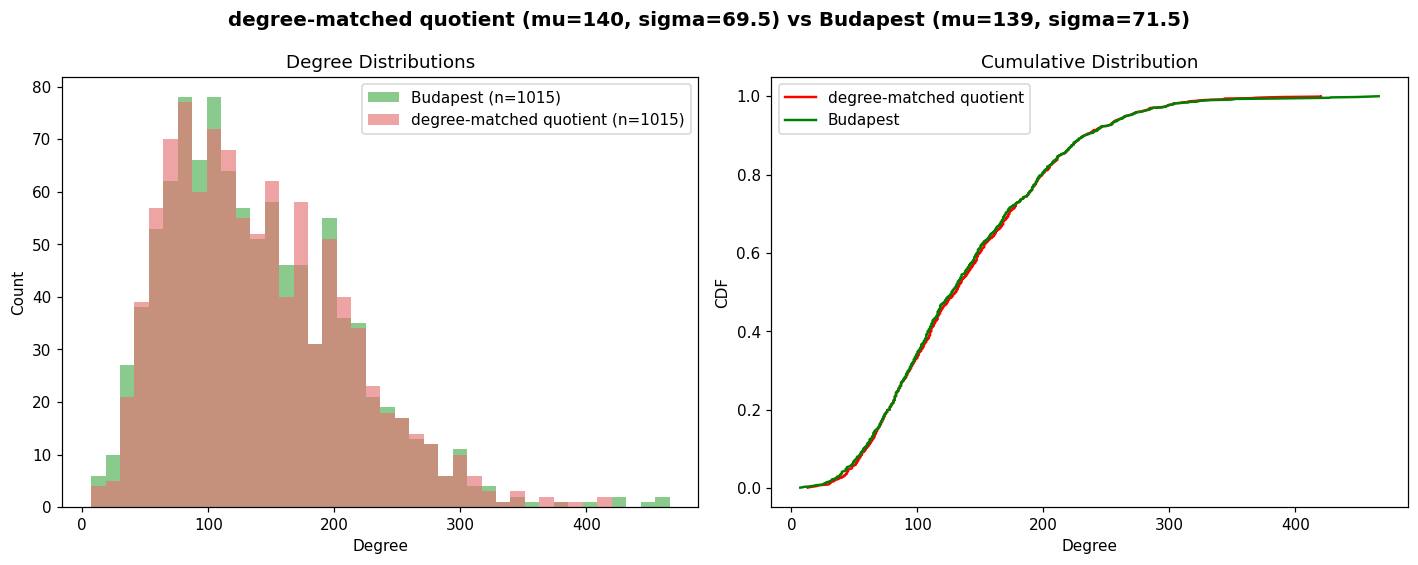
\includegraphics[width=\textwidth]{figures/degmatch_vs_budapest_degree_diff.png}
\caption{Degree comparison for the final strict quotient and Budapest.  The final degree-profile adjustment produces a close distributional match (\(KS=0.0187\)) without assigning anatomical correspondence between individual nodes.}
\label{fig:final-degree-budapest}
\end{figure}

\begin{figure}[t]
\centering
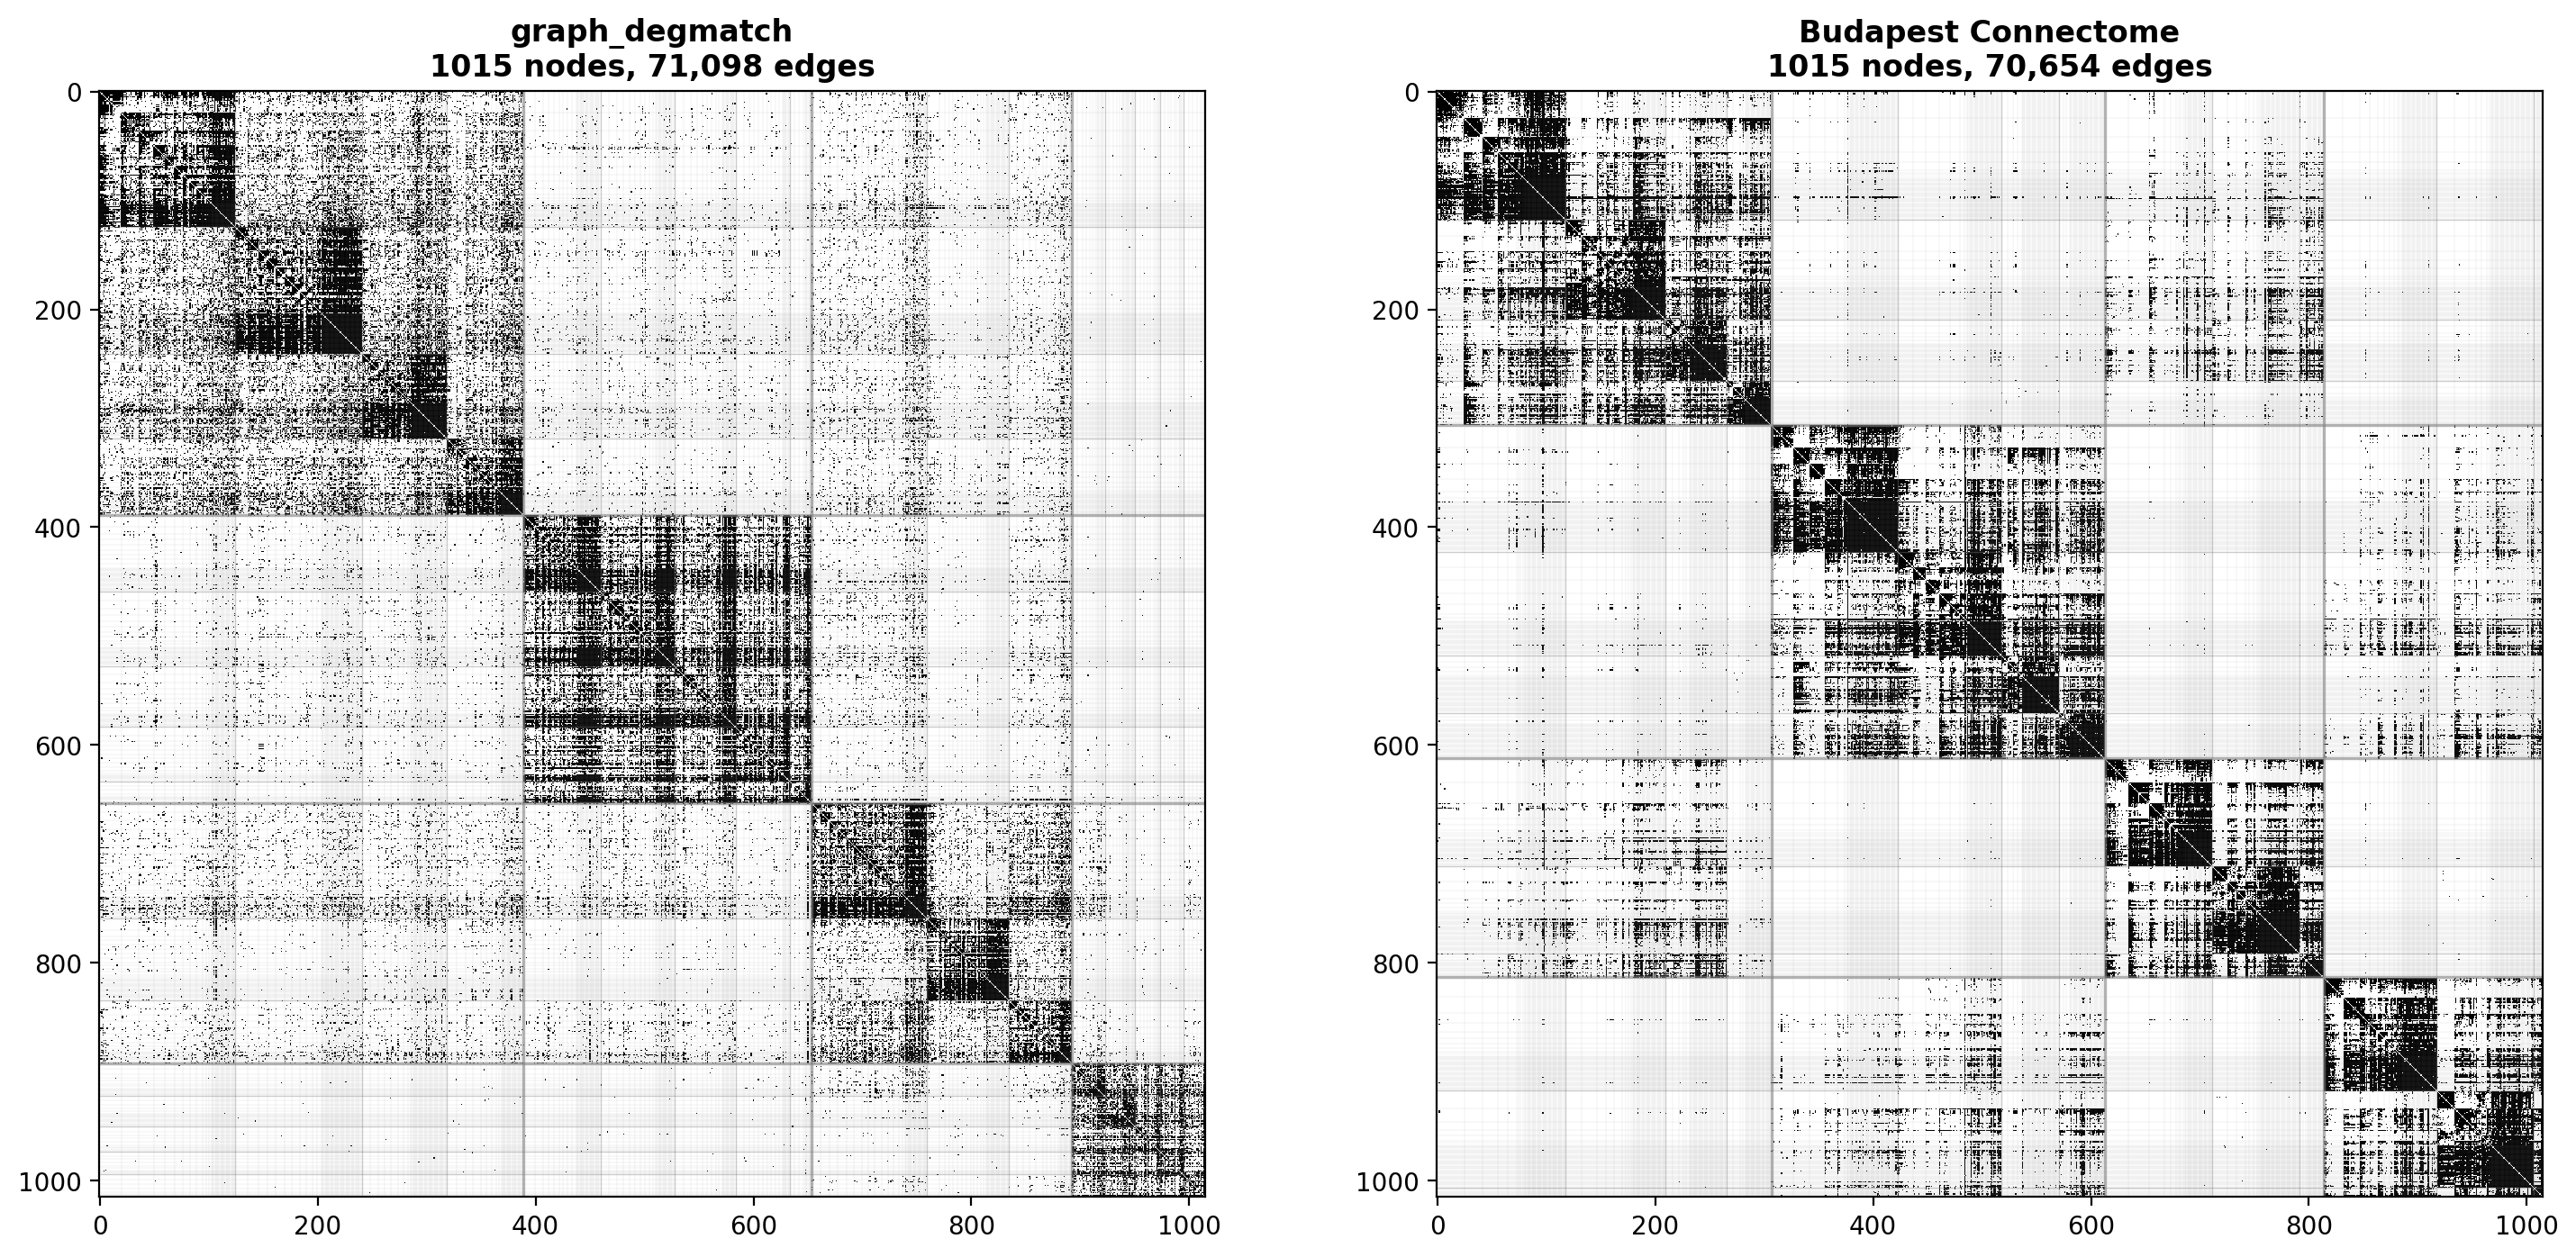
\includegraphics[width=\textwidth]{figures/degmatch_vs_budapest.png}
\caption{Community-ordered adjacency matrices of the final strict quotient (left) and the Budapest Reference Connectome (right), both with \(n=1{,}015\).  The constructed graph is the complete strict collapse of the final relocation substrate under the fixed community-derived causal partition.  Budapest shows a stronger bilateral large-scale organization that is absent from the construction.}
\label{fig:final-adjacency-budapest}
\end{figure}

\subsubsection{Nine-criterion audit}
Against \(1{,}000\) degree-preserving nulls, the final quotient passes all
nine scored criteria.  The score denotes criterion-level agreement rather
than numerical identity.

\begin{table}[H]
\centering
\small
\begin{tabularx}{\textwidth}{p{0.31\textwidth}Xc}
\toprule
Criterion & Final quotient & Verdict\\
\midrule
Clustering enriched & \(C=0.4724\), \(2.198\times\) null & PASS\\
Path length near random & \(L=1.9811\), \(1.063\times\) null & PASS\\
Small-worldness & \(\sigma_{\rm dp}=1.918\) & PASS\\
Modularity enriched & \(Q=0.4908\), \(8.00\times\) null & PASS\\
Global efficiency near random & \(E_{\rm glob}=0.5492\), \(0.966\times\) null & PASS\\
Local efficiency enriched & \(E_{\rm loc}=0.7304\), \(1.216\times\) null & PASS\\
Connector hubs & participation-based connector structure present & PASS\\
Rich-club organization & \(272\) significant thresholds; longest run \(272\) & PASS\\
Multi-resolution VI stability & stable modular scale present & PASS\\
\midrule
\multicolumn{2}{l}{\textbf{Overall score: \(9/9\).}} & \(9/9\)\\
\bottomrule
\end{tabularx}
\caption{Nine-criterion audit of the final strict quotient.  All comparisons use the stated degree-preserving null framework; the \(9/9\) result does not imply numerical identity with Budapest.}
\label{tab:final-quotient-audit}
\end{table}

Descriptive box-covering scaling is not scored at this dense scale.  Under the
same descriptive check, neither the final quotient nor Budapest supports a
clean fractal-scaling interpretation.

\subsubsection{Six static graph tests}
The final quotient is also compared with Budapest on degree distribution, hop
plot, singular-value scree, network value, triangle participation, and
effective diameter.  Its six-test mean normalized error is \(0.3033\), with
degree-distribution \(KS=0.0187\).  The degree and cumulative network-value
profiles are close; the largest residual is spectral.

\begin{figure}[p]
\centering
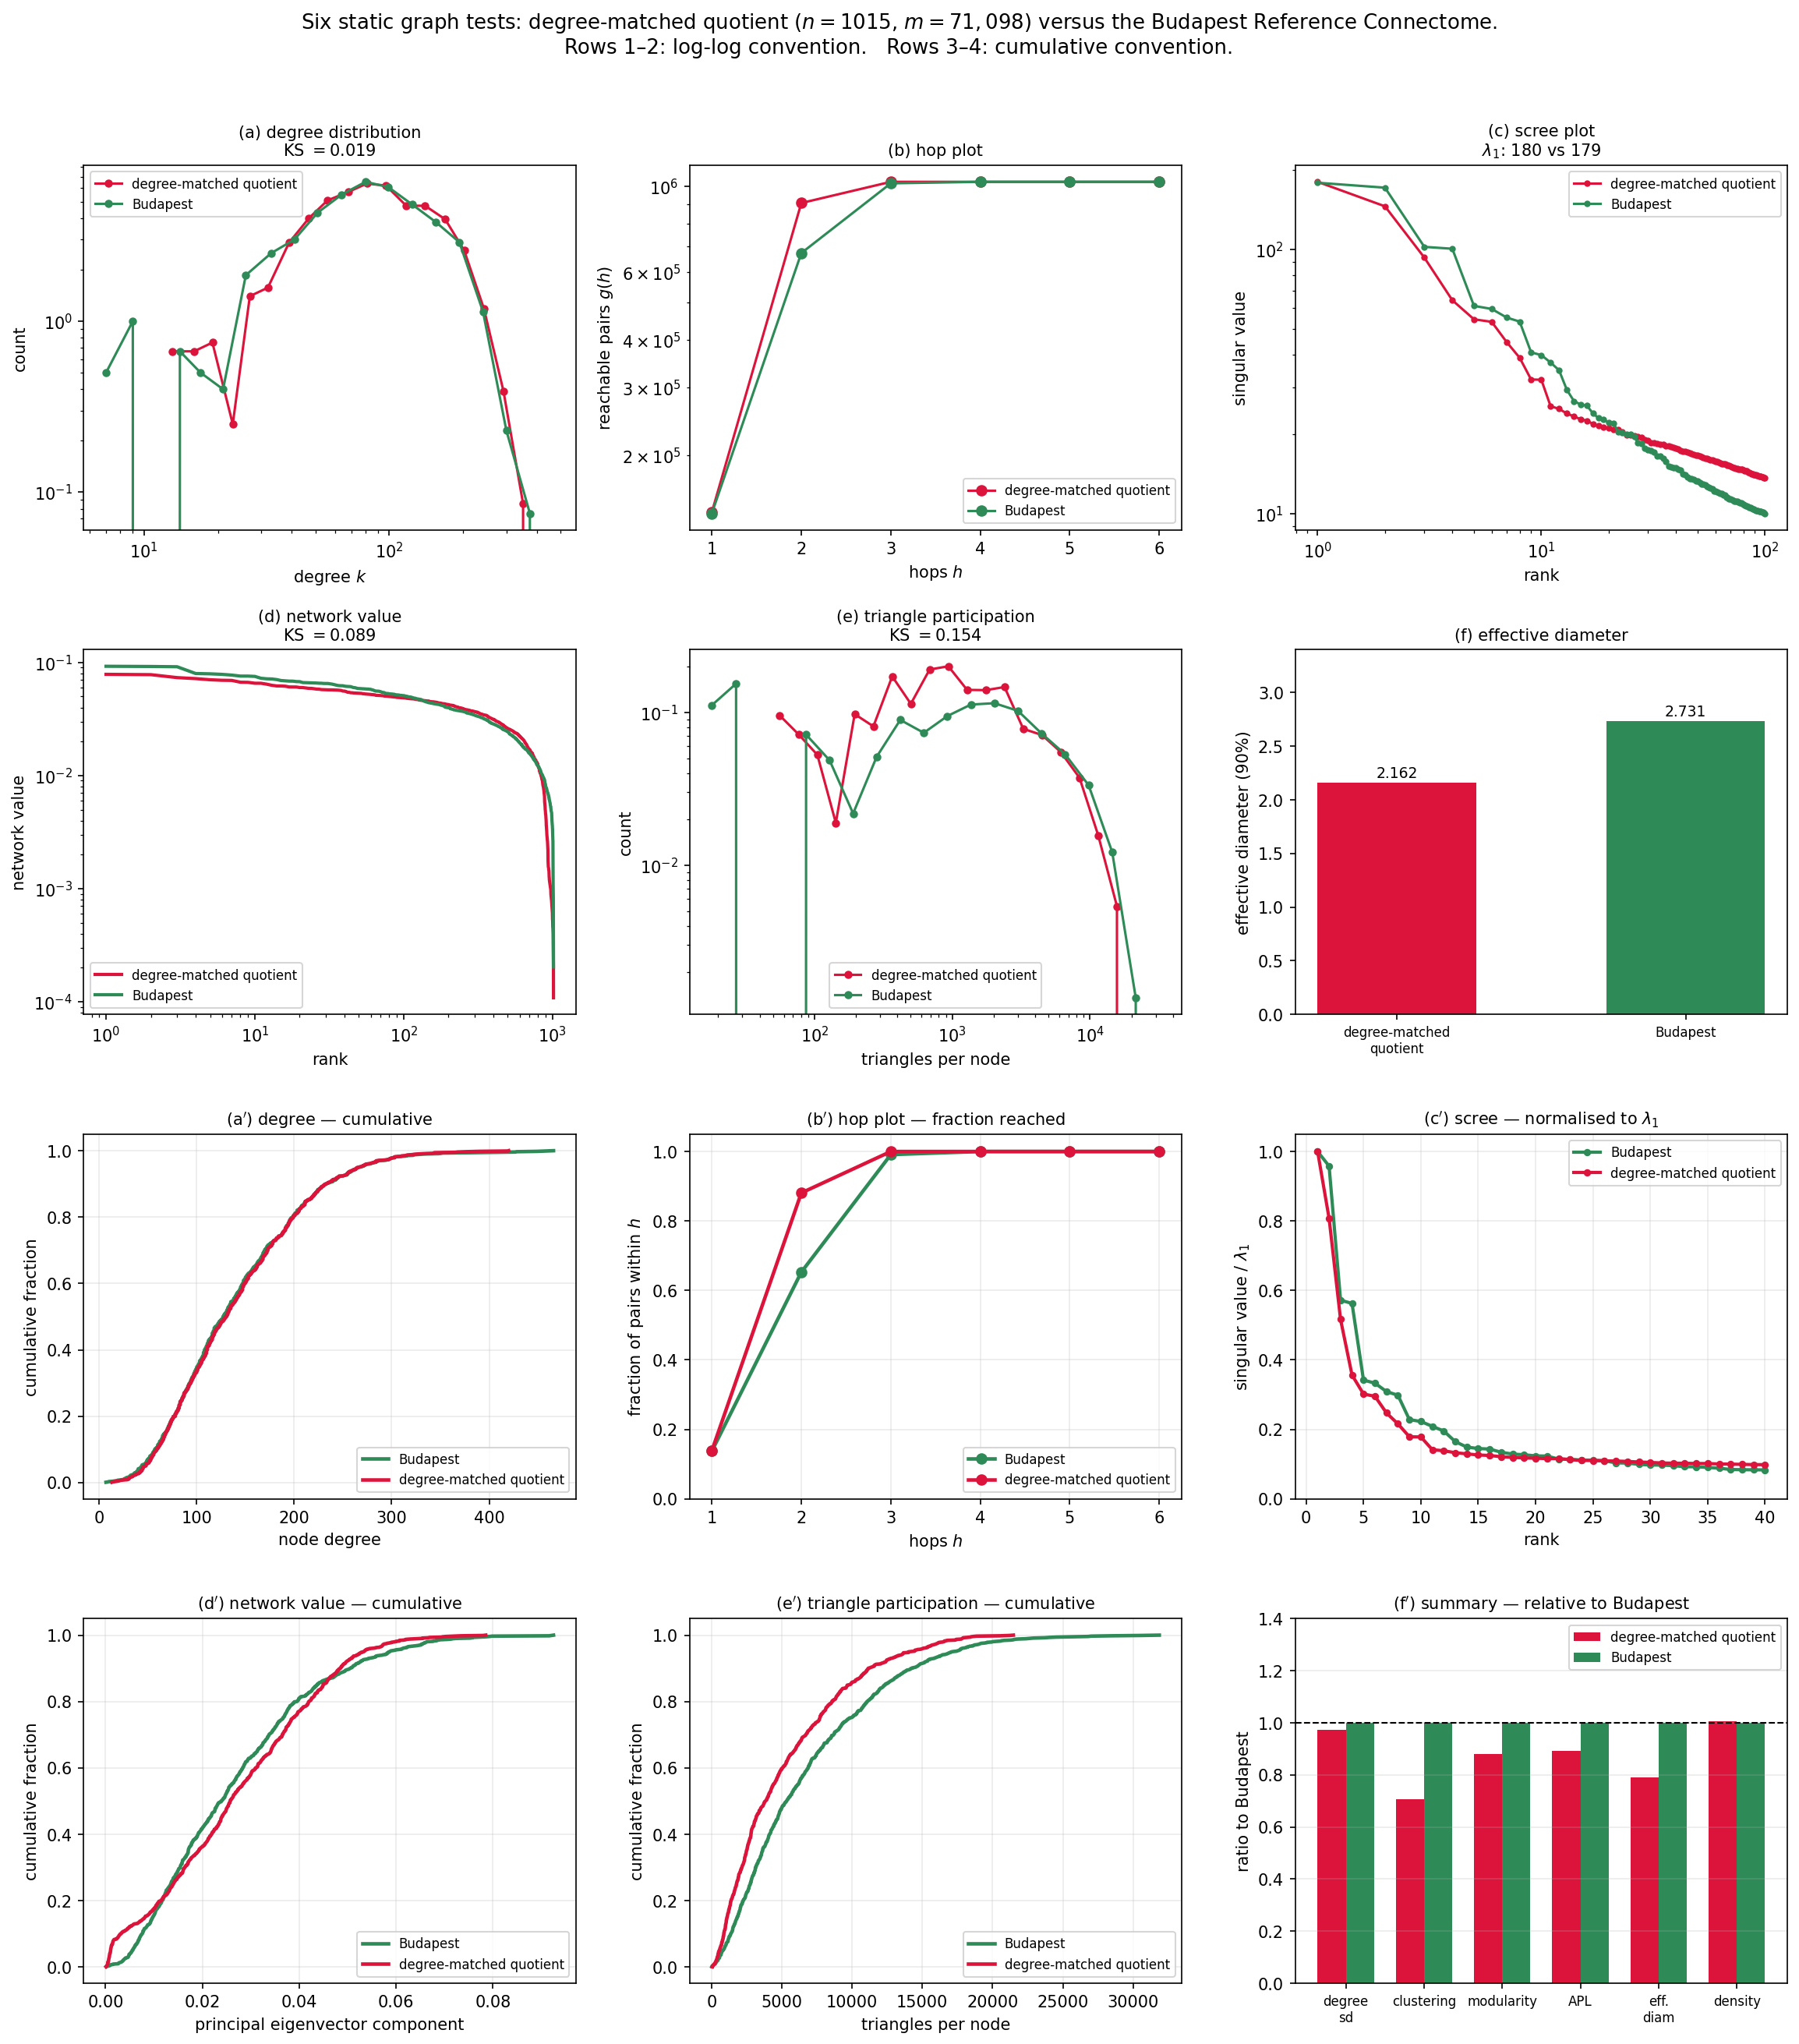
\includegraphics[width=\textwidth,height=0.78\textheight,keepaspectratio]{figures/graph_tests_degmatch.png}
\captionsetup{font=small}
\caption{Six static graph tests comparing the final strict quotient (\(n=1{,}015\), \(m=71{,}098\)) with Budapest (\(n=1{,}015\), \(m=70{,}654\)).  Rows 1--2 use the log--log convention and rows 3--4 show cumulative versions.  The degree match is especially close; the principal residual difference is spectral.}
\label{fig:graph-tests}
\end{figure}

\subsubsection{Rich-club organization}
Using \(1{,}000\) degree-preserving nulls, the \(\geq20\)-node threshold
floor, and \(p<0.05\), the final quotient has \(272\) significant degree
thresholds in one consecutive run of length \(272\).  Budapest has \(212\)
significant thresholds, also in one run.

\begin{figure}[t]
\centering
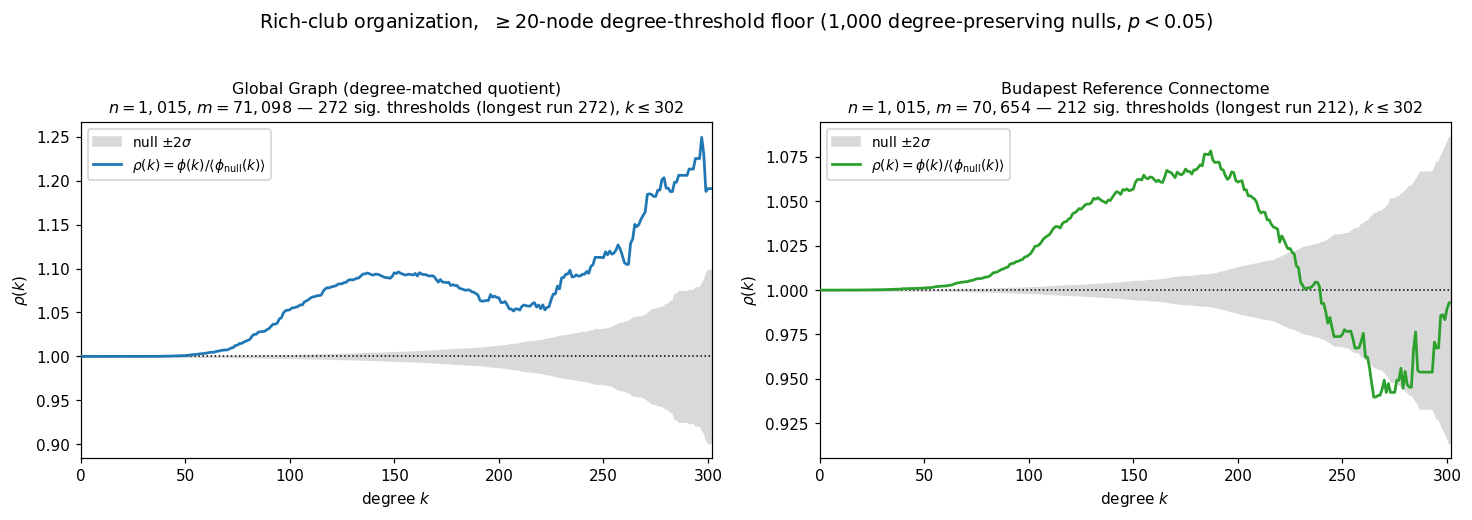
\includegraphics[width=\textwidth]{figures/richclub_rho_degmatch_vs_budapest.png}
\caption{Normalized rich-club coefficient for the final strict quotient (left) and Budapest (right), each evaluated against \(1{,}000\) degree-preserving null graphs and restricted to thresholds retaining at least \(20\) nodes.  The final quotient has a significant run of length \(272\), compared with \(212\) for Budapest.}
\label{fig:richclub-rho}
\end{figure}

\subsubsection{Complexity, spectral, and controllability diagnostics}
These quantities were not individual fitting targets and are reported as
descriptive comparisons.

\begin{table}[H]
\centering
\small
\begin{tabular}{lcc}
\toprule
Measure & Final quotient & Budapest\\
\midrule
\(\log_{10}\) Estrada index & \(78.34\) & \(77.72\)\\
Graph energy / \(n\) & \(7.009\) & \(5.693\)\\
Kirchhoff index / \(n^2\) & \(0.00985\) & \(0.01053\)\\
Off-diagonal complexity & \(5.318\) & \(5.406\)\\
Degree entropy & \(5.410\) & \(5.405\)\\
\(\lambda_{\max}/\langle d\rangle\) & \(1.288\) & \(1.285\)\\
Hoffman bound & \(6.612\) & \(7.908\)\\
Random-walk eigengap & \(0.0938\) & \(0.0197\)\\
\(\log\tau(G)/n\) & \(4.791\) & \(4.774\)\\
Average controllability & \(1.0932\) & \(1.1004\)\\
\bottomrule
\end{tabular}
\caption{Selected complexity, spectral, and controllability diagnostics.  Resistance-based, spanning-tree, leading-eigenvalue, average-controllability, off-diagonal-complexity, and degree-entropy quantities are close, while the random-walk eigengap remains different.}
\label{tab:final-complexity}
\end{table}

The clearest unresolved large-scale feature is bilateral organization.  The
Budapest graph has a near-degenerate leading spectral pair
\(\lambda_1=178.9\), \(\lambda_2=171.4\) and a top-level community pattern
\(307/306/201/201\) that naturally separates into approximately balanced
halves.  The final quotient instead has top-level sizes
\(389/265/239/122\) and no paired organization.  The \(1{,}015\)-node match is
therefore distributional rather than anatomical; bilateral organization
would require additional anatomical or spatial information not present in
the substrate.


\begin{thebibliography}{99}

\bibitem{Szalkai2015Budapest}
B.~Szalkai, C.~Kerepesi, B.~Varga, and V.~Grolmusz,
``The Budapest Reference Connectome Server v2.0,''
\emph{Neuroscience Letters}, 595:60--62, 2015.
doi:10.1016/j.neulet.2015.03.071.

\bibitem{Szalkai2017Budapest}
B.~Szalkai, C.~Kerepesi, B.~Varga, and V.~Grolmusz,
``Parameterizable consensus connectomes from the Human Connectome Project:
the Budapest Reference Connectome Server v3.0,''
\emph{Cognitive Neurodynamics}, 11(1):113--116, 2017.
doi:10.1007/s11571-016-9407-z.

\bibitem{VargaGrolmusz2021Braingraph}
B.~Varga and V.~Grolmusz,
``The braingraph.org database with more than 1000 robust human connectomes
in five resolutions,''
\emph{Cognitive Neurodynamics}, 15:915--919, 2021.
doi:10.1007/s11571-021-09670-5.

\bibitem{LeskovecKronecker2010} 
J.~Leskovec, D.~Chakrabarti, J.~Kleinberg, C.~Faloutsos, and
Z.~Ghahramani,
``Kronecker graphs: An approach to modeling networks,''
\emph{Journal of Machine Learning Research}, 11:985--1042, 2010.

\bibitem{Blondel2008}
V.~D.~Blondel, J.-L.~Guillaume, R.~Lambiotte, and E.~Lefebvre,
``Fast unfolding of communities in large networks,''
\emph{Journal of Statistical Mechanics: Theory and Experiment},
2008:P10008, 2008.

\bibitem{RubinovSporns2010}
M.~Rubinov and O.~Sporns,
``Complex network measures of brain connectivity: uses and interpretations,''
\emph{NeuroImage}, 52(3):1059--1069, 2010.

\bibitem{FornitoZalBull2016}
A.~Fornito, A.~Zalesky, and E.~T.~Bullmore,
\emph{Fundamentals of Brain Network Analysis},
Academic Press, San Diego, 2016.

\bibitem{SizemoreCliques2018}
A.~E. Sizemore, C.~Giusti, A.~Kahn, J.~M. Vettel, R.~F. Betzel,
and D.~S. Bassett,
``Cliques and cavities in the human connectome,''
\emph{Journal of Computational Neuroscience}, 44:115--145, 2018.

\bibitem{MiloMotifs2002}
R.~Milo, S.~Shen-Orr, S.~Itzkovitz, N.~Kashtan, D.~Chklovskii,
and U.~Alon,
``Network motifs: simple building blocks of complex networks,''
\emph{Science}, 298:824--827, 2002.

\bibitem{KimWilhelm2008ComplexGraph}
J. Kim and T. Wilhelm,
``What is a complex graph?''
\emph{Physica A: Statistical Mechanics and its Applications},
387(11):2637--2652, 2008.

\bibitem{PrzuljGraphlets2004}
N.~Pr\v{z}ulj, D.~G. Corneil, and I.~Jurisica,
``Modeling interactome: scale-free or geometric?''
\emph{Bioinformatics}, 20:3508--3515, 2004.

\bibitem{SpornsKotterMotifs2004}
O.~Sporns and R.~K\"otter,
``Motifs in brain networks,''
\emph{PLoS Biology}, 2:e369, 2004.

\bibitem{Farahani2019}
F.~V.~Farahani, W.~Karwowski, and N.~R.~Lighthall,
``Application of graph theory for identifying connectivity patterns in human brain networks: a systematic review,''
\emph{Frontiers in Neuroscience}, 13:585, 2019.

\bibitem{MaslovSneppen2002}
S.~Maslov and K.~Sneppen,
``Specificity and stability in topology of protein networks,''
\emph{Science}, 296(5569):910--913, 2002.

\bibitem{VasaMisic2022}
F.~Vasa and B.~Misic,
``Null models in network neuroscience,''
\emph{Nature Reviews Neuroscience}, 23(8):493--504, 2022.

\bibitem{WattsStrogatz1998}
D.~J.~Watts and S.~H.~Strogatz,
``Collective dynamics of small-world networks,''
\emph{Nature}, 393(6684):440--442, 1998.

\bibitem{HumphriesGurney2008}
M.~D.~Humphries and K.~Gurney,
``Network small-world-ness: a quantitative method for determining canonical network equivalence,''
\emph{PLoS ONE}, 3(4):e0002051, 2008.

\bibitem{NewmanGirvan2004}
M.~E.~J.~Newman and M.~Girvan,
``Finding and evaluating community structure in networks,''
\emph{Physical Review E}, 69(2):026113, 2004.

\bibitem{ClausetNewmanMoore2004}
A.~Clauset, M.~E.~J.~Newman, and C.~Moore,
``Finding community structure in very large networks,''
\emph{Physical Review E}, 70:066111, 2004.

\bibitem{LatoraMarchiori2001}
V.~Latora and M.~Marchiori,
``Efficient behavior of small-world networks,''
\emph{Physical Review Letters}, 87(19):198701, 2001.

\bibitem{IturriaMedina2008}
Y.~Iturria-Medina, R.~C.~Sotero, E.~J.~Canales-Rodriguez,
Y.~Aleman-Gomez, and L.~Melie-Garcia,
``Studying the human brain anatomical network via diffusion-weighted MRI and graph theory,''
\emph{NeuroImage}, 40(3):1064--1076, 2008.

\bibitem{Guimera2005}
R.~Guimera and L.~A.~N.~Amaral,
``Functional cartography of complex metabolic networks,''
\emph{Nature}, 433:895--900, 2005.

\bibitem{Colizza2006}
V.~Colizza, A.~Flammini, M.~A.~Serrano, and A.~Vespignani,
``Detecting rich-club ordering in complex networks,''
\emph{Nature Physics}, 2:110--115, 2006.

\bibitem{vandenHeuvel2011}
M.~P.~van~den Heuvel and O.~Sporns,
``Rich-club organization of the human connectome,''
\emph{Journal of Neuroscience}, 31(44):15775--15786, 2011.

\bibitem{Meila2007}
M.~Meila,
``Comparing clusterings: an information based distance,''
\emph{Journal of Multivariate Analysis}, 98(5):873--895, 2007.

\bibitem{Betzel2017modular}
R.~F.~Betzel, J.~D.~Medaglia, L.~Papadopoulos, G.~L.~Baum,
R.~Gur, R.~Gur, R.~Roalf, T.~D.~Satterthwaite, and D.~S.~Bassett,
``The modular organization of human anatomical brain networks: accounting for the cost of wiring,''
\emph{Network Neuroscience}, 1(1):42--68, 2017.

\bibitem{Song2005}
C.~Song, S.~Havlin, and H.~A.~Makse,
``Self-similarity of complex networks,''
\emph{Nature}, 433:392--395, 2005.

\bibitem{Song2007memb}
C.~Song, L.~K.~Gallos, S.~Havlin, and H.~A.~Makse,
``How to calculate the fractal dimension of a complex network: the box covering algorithm,''
\emph{Journal of Statistical Mechanics}, 2007:P03006, 2007.

\bibitem{XueBogdan2017}
Y.~Xue and P.~Bogdan,
``Reliable multi-fractal characterization of weighted complex networks: algorithms and implications,''
\emph{Scientific Reports}, 7:7487, 2017.

\bibitem{Szalkai2018Lobes}
B.~Szalkai, B.~Varga, and V.~Grolmusz,
``Comparing advanced graph-theoretical parameters of the connectomes
of the lobes of the human brain,''
\emph{Cognitive Neurodynamics}, 12(6):549--559, 2018.

\bibitem{Szalkai2021GraphMind}
B.~Szalkai, B.~Varga, and V.~Grolmusz,
``The graph of our mind,''
\emph{Brain Sciences}, 11(3):342, 2021.

\bibitem{Hoffman1970}
A.~J.~Hoffman,
``On eigenvalues and colorings of graphs,''
in B.~Harris, editor,
\emph{Graph Theory and its Applications},
Academic Press, New York, pp.~79--91, 1970.

\bibitem{Kirchhoff1847}
G.~Kirchhoff,
``Ueber die Aufl\"osung der Gleichungen, auf welche man bei der
Untersuchung der linearen Vertheilung galvanischer Str\"ome gef\"uhrt
wird,''
\emph{Annalen der Physik und Chemie}, 72(12):497--508, 1847.

\bibitem{Fiedler1973}
M.~Fiedler,
``Algebraic connectivity of graphs,''
\emph{Czechoslovak Mathematical Journal}, 23(2):298--305, 1973.

\bibitem{Edmonds1965}
J.~Edmonds,
``Paths, trees, and flowers,''
\emph{Canadian Journal of Mathematics}, 17:449--467, 1965.

\bibitem{Kruskal1956}
J.~B.~Kruskal,
``On the shortest spanning subtree of a graph and the traveling salesman
problem,''
\emph{Proceedings of the American Mathematical Society}, 7(1):48--50,
1956.

\bibitem{Estrada2000}
E.~Estrada,
``Characterization of 3D molecular structure,''
\emph{Chemical Physics Letters}, 319:713--718, 2000.

\bibitem{Gutman1978}
I.~Gutman, ``The energy of a graph,''
\emph{Ber.\ Math.-Statist.\ Sekt.\ Forschungsz.\ Graz}, 103:1--22, 1978.

\bibitem{KleinRandic1993}
D.~J.~Klein and M.~Randi\'{c},
``Resistance distance,''
\emph{Journal of Mathematical Chemistry}, 12:81--95, 1993.


\bibitem{Claussen2007}
J.~C.~Claussen,
``Off-diagonal complexity: a computationally quick complexity measure
for graphs and networks,''
\emph{Physica A: Statistical Mechanics and its Applications},
375(1):365--373, 2007.

\bibitem{Gu2015Controllability}
S.~Gu, F.~Pasqualetti, M.~Cieslak, Q.~K.~Telesford, A.~B.~Yu,
A.~E.~Kahn, J.~D.~Medaglia, J.~M.~Vettel, M.~B.~Miller,
S.~T.~Grafton, and D.~S.~Bassett,
``Controllability of structural brain networks,''
\emph{Nature Communications}, 6:8414, 2015.

\bibitem{BetzelBassett2017}
R.~F. Betzel and D.~S. Bassett,
``Multi-scale brain networks,''
\emph{NeuroImage},
vol.~160, pp.~73--83, 2017.

\end{thebibliography}



\end{document}